\chapter{Coupled Lines with Resonance}
\label{chap:coupled-lines-resonance}
\index{coupled lines}
\index{resonance!parallel overhead lines}
\index{line transposition}
\index{inductive compensation}

\section{General}
\label{sec:coupled-lines-general}

This chapter investigates two electromagnetically coupled
\SI{400}{\kilo\volt} overhead lines on a common Danube-type tower. 
The capacitive reactive power of the two lines is compensated by an inductive choke. We will examine the case where the compensation is near ideal—that is, where the inductive reactive power of the choke compensates for the capacitive reactive power of the line.
The following cases are simulated (Line 1 is always energized):

\begin{itemize}
	\item \texttt{Line 2 is open (lines are untransposed)},
	\item \texttt{Line 2 is open (lines are transposed)},
	\item \texttt{Line 2 is initially grounded and then ungrounded},
	\item \texttt{Line 2 is initially energized and then switched off},
	\item \texttt{Line 2 is initially energized and then switched off without a com-pensating reactor}
\end{itemize}

\section{Circuit design}
The total
line length is approximately \SI{9.75}{\kilo\metre}. Mutual inductances and
capacitances couple the circuits even when one line is disconnected at both
ends.

The per-kilometre inductance and capacitance matrices of the coupled line were calculated with ATP
and then stored in \texttt{line\_coupled.lib}.
The Excel file Lines\_and\_cables.xlsx assists with conversion to LTspice library code.

Each line is almost fully compensated by an shunt reactor
element, \texttt{l\_batt}. Near-exact compensation creates an important
operating condition: if line 1 is energized while line 2 is open at both ends,
the mutual coupling can excite a resonance and produce very high voltages on
the disconnected line.

\section{Determining the Compensation Rating}
\label{sec:coupled-line-compensation-rating}

Use \texttt{Coupled\_lines\_resonance\_TRAN.asc}. Save a working copy as
\texttt{test.asc}, remove the compensation elements, and run the transient
simulation. Measure the three phase reactive powers with
\texttt{qmeter\_uvw\_sgn}. The results are approximately

\begin{align}
Q_R&=\SI{-2.02}{\mega\varunit},&
Q_S&=\SI{-2.40}{\mega\varunit},&
Q_T&=\SI{-2.37}{\mega\varunit}.
\end{align}

The total capacitive reactive power is therefore approximately
\SI{-6.8}{\mega\varunit}. A compensation rating of
\SI{+6}{\mega\varunit} is selected for each line, leaving the system close to,
but not exactly at, resonance.

At \SI{400}{\kilo\volt}, the corresponding balanced three-phase current is

\begin{calculation}{Current of the \SI{6}{\mega\varunit} compensation reactor}{calculation71}
\begin{align}
I_{\mathrm{rms}}
 &=\frac{Q}{\sqrt{3}U_{\mathrm{LL}}}
   =\frac{\SI{6}{\mega\varunit}}
          {\sqrt{3}\cdot\SI{400}{\kilo\volt}}
   \approx\SI{8.66}{\ampere},\\
\widehat I&=\sqrt{2}\,I_{\mathrm{rms}}
   \approx\boxed{\SI{12.2}{\ampere}}.
\end{align}
\end{calculation}

\section{Line 1 Energized and Line 2 Open: Untransposed Lines} figures: \ref{fig:figure72}-\ref{fig:figure73}  (simulation-file: same name as the heading)
\label{sec:coupled-lines-open-untransposed}

Line 1 is supplied by a source with an exponential voltage startup, while line 2 remains
open at both ends. The open-line voltages exhibit a slow beat and approach
their final values after approximately \SI{2}{\second}.

Phase A of line 2 has the highest voltage, with transient peaks near
\SI{500}{\kilo\volt}, corresponding to approximately
\SI{350}{\kilo\volt} RMS. The other two phase peaks remain below
\SI{300}{\kilo\volt}. For comparison, the normal phase-voltage peak of the
energized \SI{400}{\kilo\volt} line is

\begin{equation}
\widehat U_{\mathrm{ph}}
 =\sqrt{2}\frac{U_{\mathrm{LL}}}{\sqrt{3}}
 =\sqrt{2}\frac{\SI{400}{\kilo\volt}}{\sqrt{3}} 
 \approx\SI{326.6}{\kilo\volt} peak.
\end{equation}

The settled phase A peak on line 2 is approximately
\SI{350}{\kilo\volt}, exceeding the normal phase-voltage peak of 327 kV on line 1 with \SI{327}{\kilo\volt} . The slow
envelope is caused by the small difference between the \SI{50}{\hertz} source
frequency and a nearby natural frequency formed by the line capacitances and
the compensating \texttt{l\_batt} reactors. 

The reactor-current peaks on line 1 are approximately
\SI{12}{\ampere} in all three phases, consistent with calculation \ref{calc:calculation71}. On line 2, the peak currents are
approximately \SI{13.3}{\ampere}, \SI{6}{\ampere}, and
\SI{7}{\ampere} in phases A, B, and C, respectively. The source currents are
close to zero because the line charging current is almost compensated.

The untransposed line has strongly unequal mutual capacitances and inductances.
Consequently, the phase magnitudes and phase angles on open line 2 are highly
asymmetric, and the sum of its three phase-to-earth voltages is nonzero, with a residual sum of approximately 46 kV.

\begin{figure}[H]
	\centering
	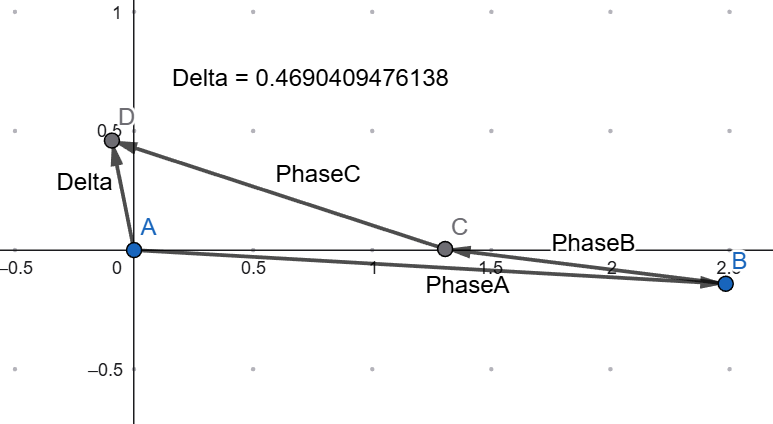
\includegraphics[width=0.8\textwidth]{figures/07_Coupled_lines_resonance/Sum_of_voltages_not_zero}
	\caption{Coupled lines resonance - Sum of voltages not zero - scale multiplied by 1e5}
	\label{fig:figure71}
\end{figure}


\begin{figure}[H]
	\centering
	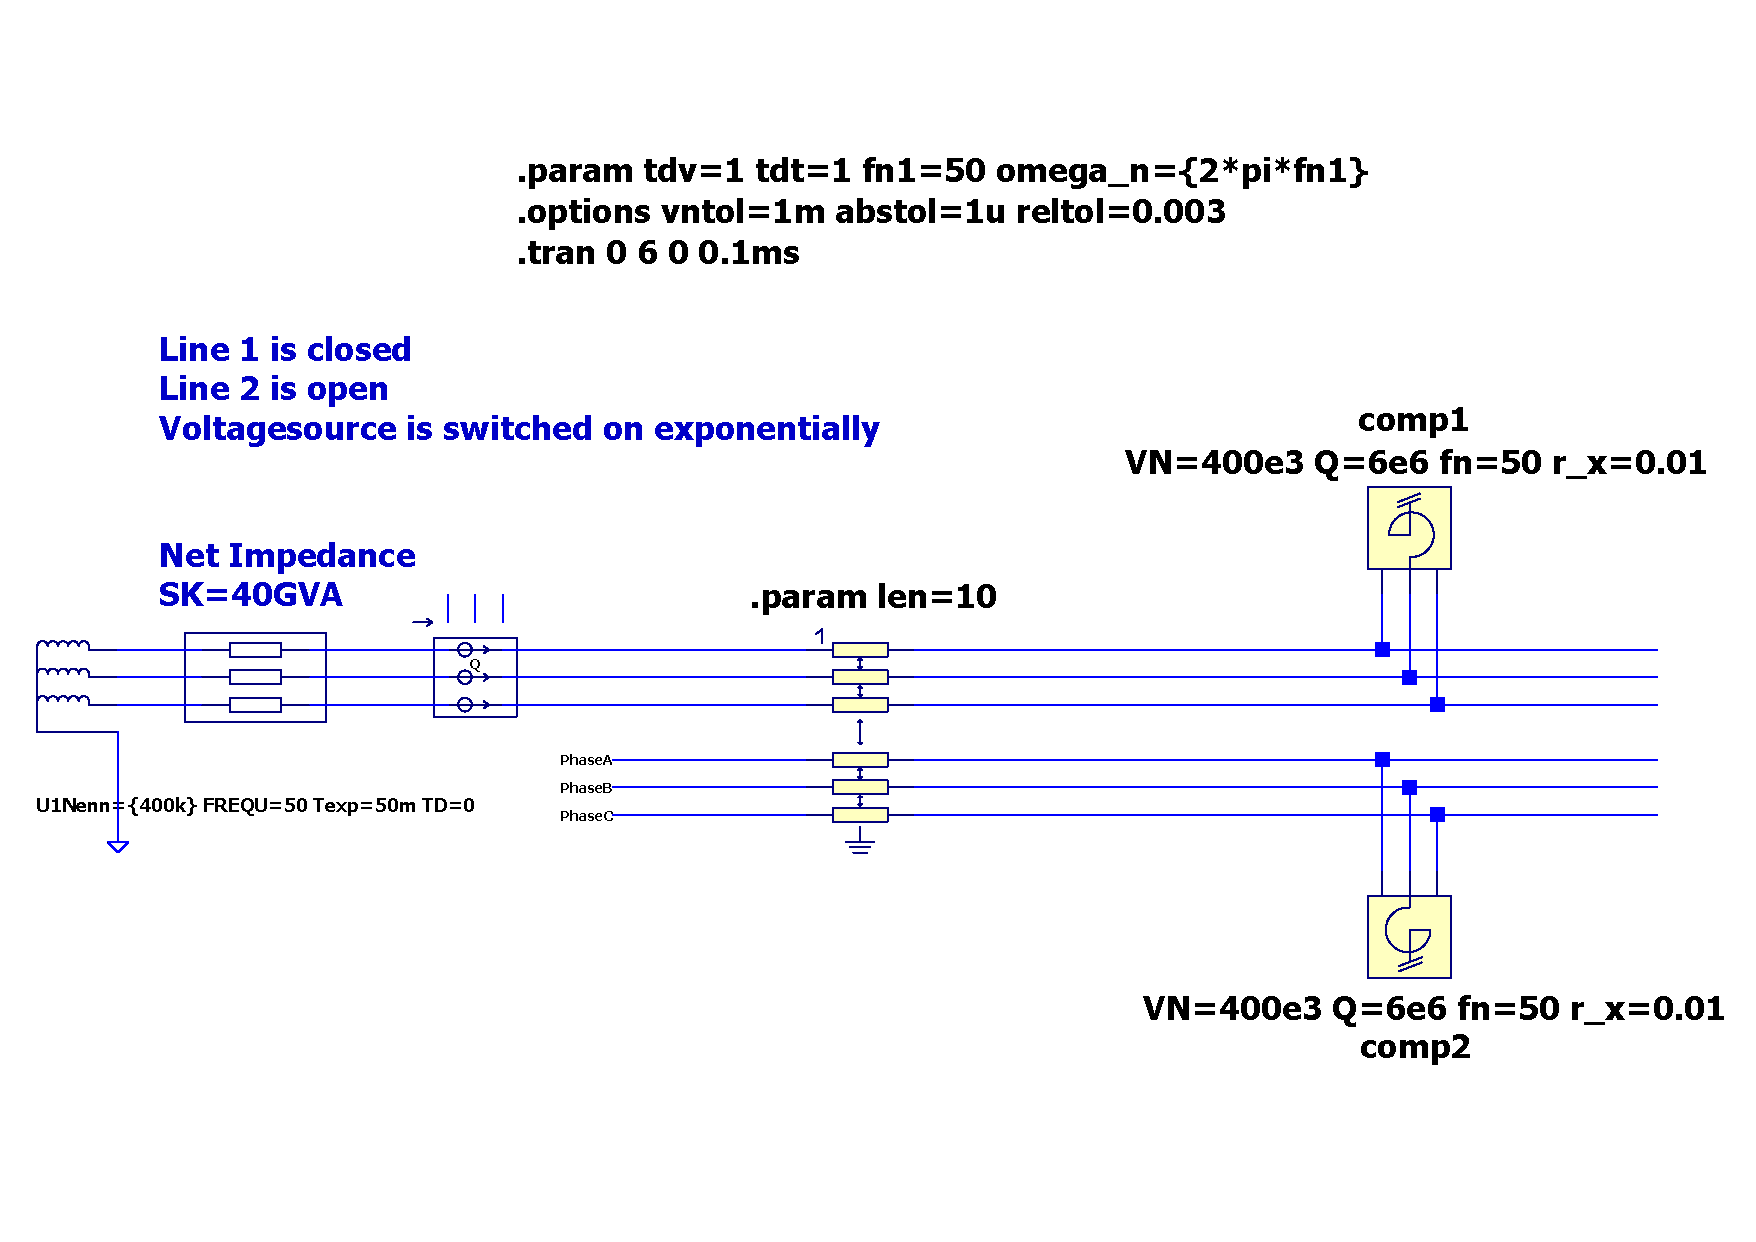
\includegraphics[width=1.0\textwidth]{figures/07_Coupled_lines_resonance/Coupled_lines_resonance_TRAN_schematic}
	\caption{Coupled lines resonance schematic - line2 is open untransposed TRAN analysis}
	\label{fig:figure72}
\end{figure}

\begin{figure}[H]
	\centering
	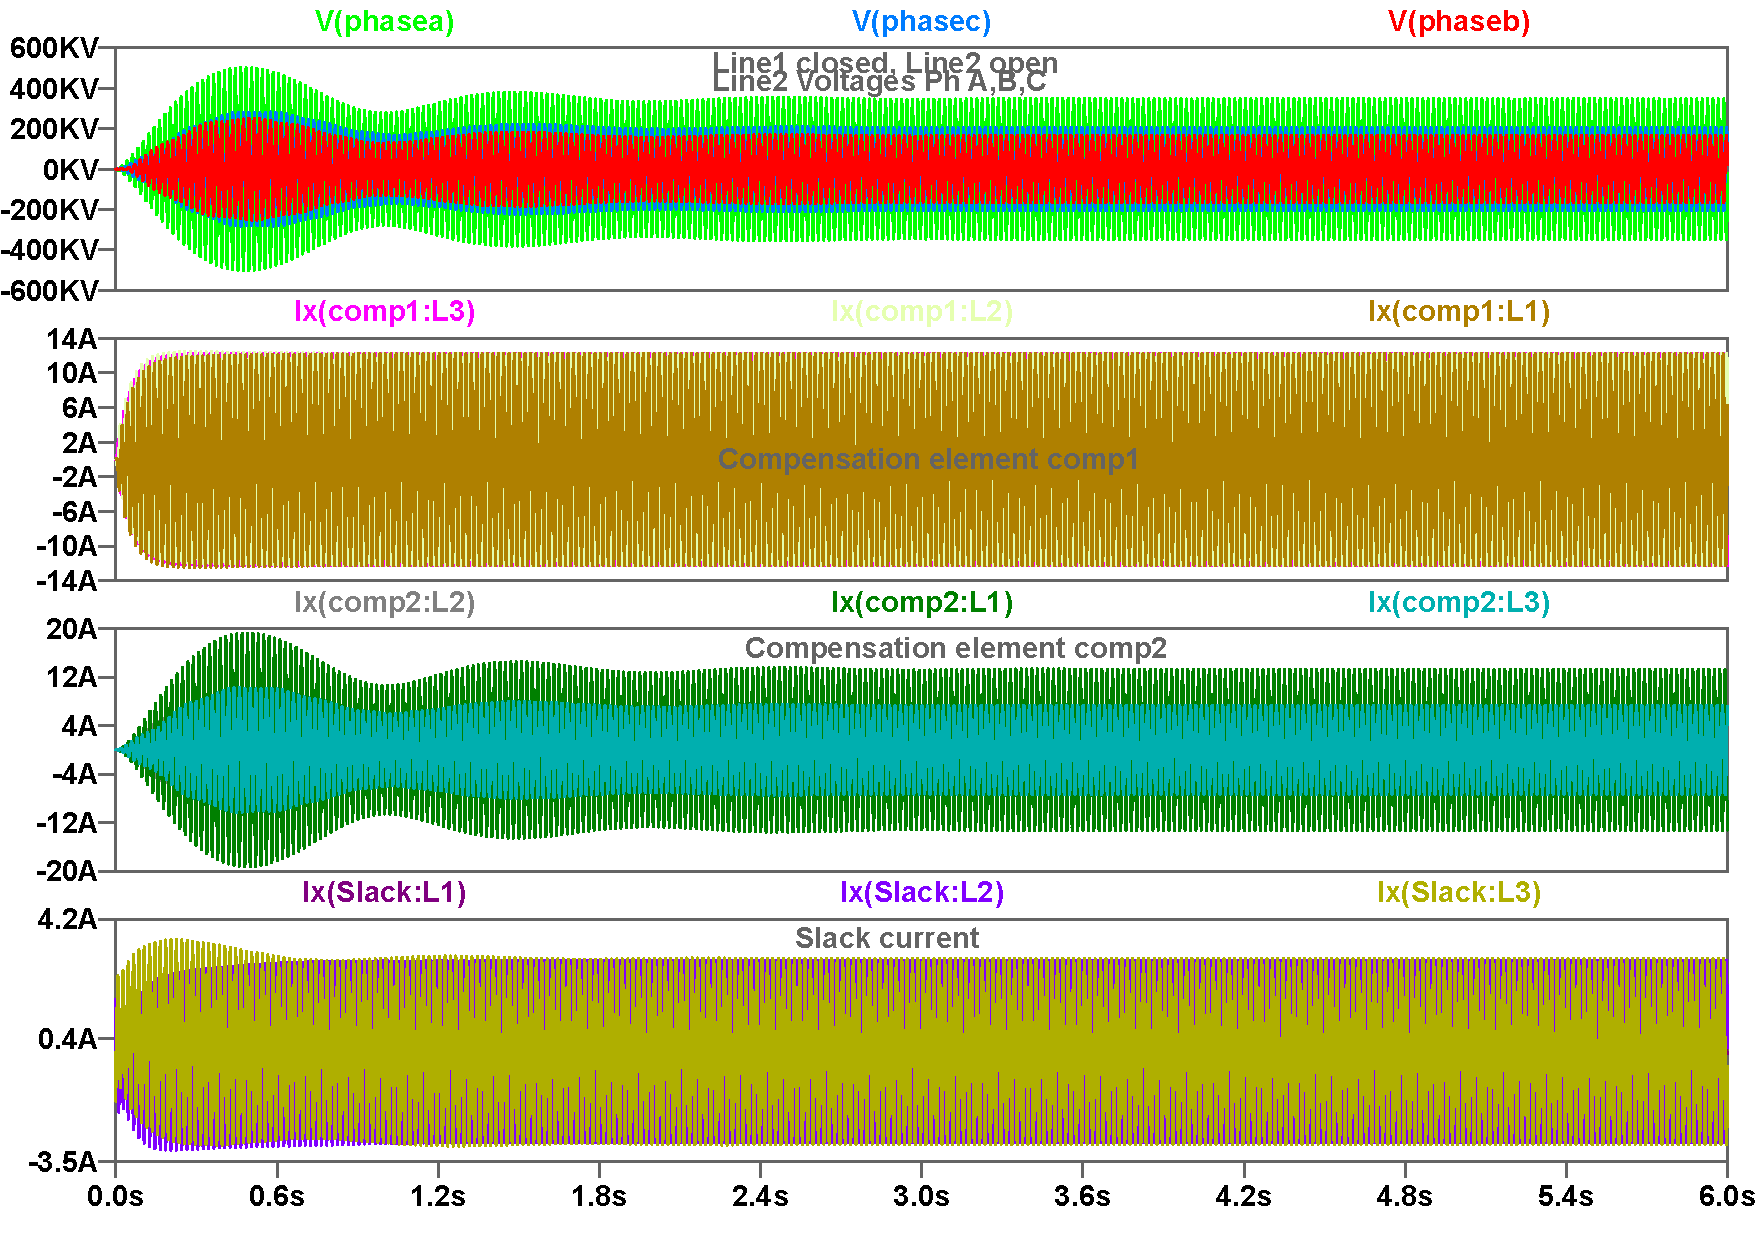
\includegraphics[width=0.90\textwidth]{figures/07_Coupled_lines_resonance/Coupled_lines_resonance_TRAN}
	\caption{Coupled lines resonance TRAN - line2 is open untransposed TRAN analysis}
	\label{fig:figure73}
\end{figure}


\section{AC Analysis of the Untransposed Open Line} figures: \ref{fig:figure74}-\ref{fig:figure75}  (simulation-file: same name as the heading) 
\label{sec:coupled-lines-ac-untransposed}

Set the vertical scale to linear by right-clicking the left axis. The principal
resonance of the open-line voltage lies near \SI{49}{\hertz}. At
\SI{50}{\hertz}, the phase-R voltage is approximately
\SI{250}{\kilo\volt} RMS, compared with the normal phase voltage of
approximately \SI{231}{\kilo\volt} RMS. This corresponds to the settled
transient value of approximately \SI{353}{\kilo\volt} peak.

A second resonance occurs near \SI{44}{\hertz}. At the main resonant peak near
\SI{49}{\hertz}, the Phase A voltage can approach approximately
\SI{1}{\mega\volt} peak. This demonstrates the sensitivity of the open coupled
line to small changes in shunt-reactor tuning.

\begin{important}{Near-resonant open-line overvoltage}{imp:coupled-line-resonance}
An open line is not necessarily de-energized when it shares a tower with an
energized line. Mutual capacitances and inductances can sustain a substantial
voltage, and near-resonant shunt compensation can amplify it far above the
normal phase voltage.
\end{important}

\subsection{Exercises}

\begin{enumerate}
\item Save the model as \texttt{test.asc} and increase the
      \texttt{l\_batt} rating until the resonant peak lies at
      \SI{50}{\hertz}. Observe the resulting voltage amplification.
\item Reduce the reactor rating to \SI{5}{\mega\varunit}. Compare the resonant
      frequency and peak magnitude with the original case.
\item Change the reactor parameter \texttt{r\_x}, which represents its ohmic
      component. Observe how increasing damping broadens and lowers the
      resonant peak.
\end{enumerate}

\section{Line 1 Energized and Line 2 Open: Transposed Lines} figures: \ref{fig:figure76}-\ref{fig:figure77}  (simulation-file: same name as the heading) 
\label{sec:coupled-lines-open-transposed}

Transposition makes the phase coupling approximately symmetrical. The three
open-line voltages therefore have equal magnitudes, and the relevant resonance
moves farther away from the power frequency.

The initial open-line peaks are approximately \SI{100}{\kilo\volt} and decay
to about \SI{70}{\kilo\volt} after \SI{2}{\second}. This is a substantially
more favourable operating condition than the untransposed case in
\cref{sec:coupled-lines-open-untransposed}.

\begin{remark}{Exercise}{imp:transposed-line-reactive-power}
	Save the model as \texttt{test.asc}, remove the \texttt{l\_batt} elements from
	both lines, and compare the phase currents and reactive powers of lines 1 and
	2. The transposed model should produce nearly symmetrical phase results.
\end{remark}

\begin{figure}[H]
	\centering
	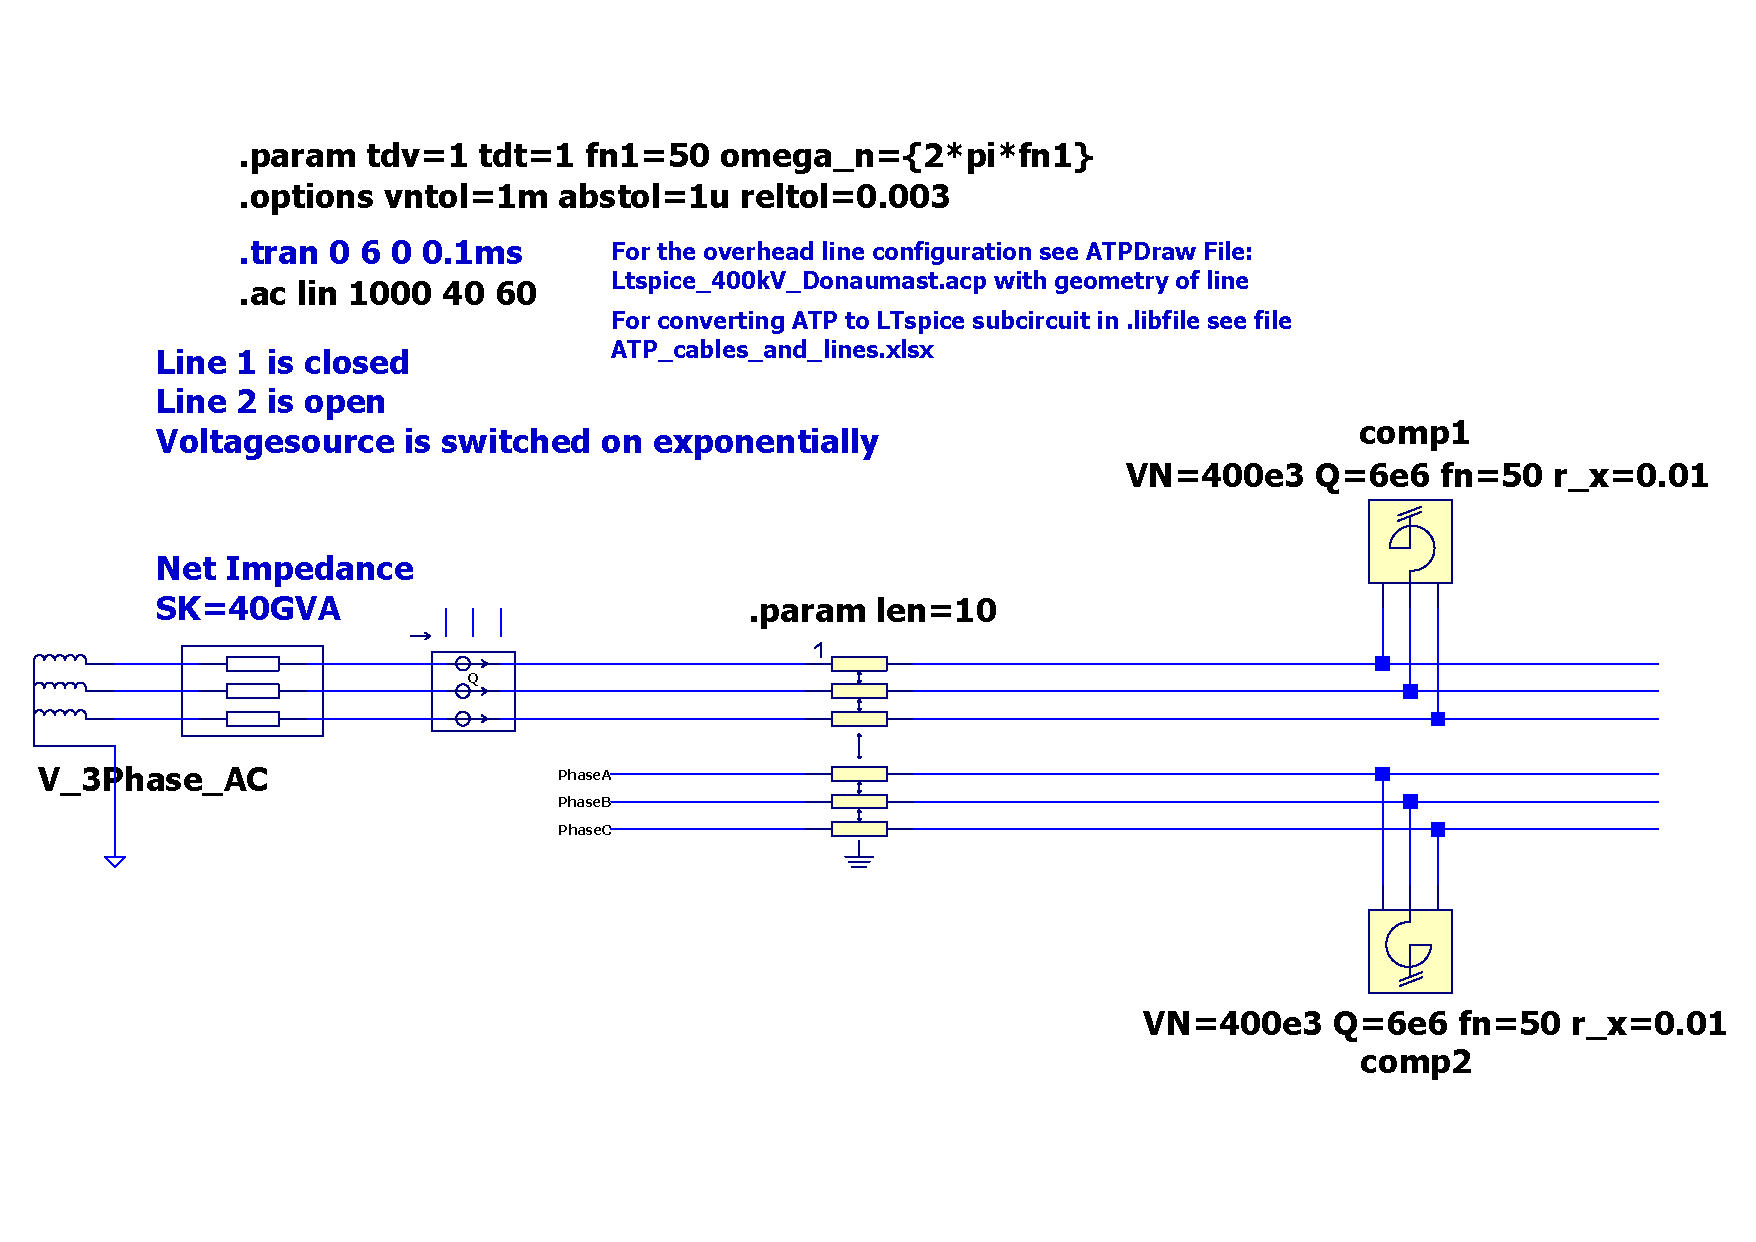
\includegraphics[width=1.0\textwidth]{figures/07_Coupled_lines_resonance/Coupled_lines_resonance_AC_schematic}
	\caption{Coupled lines resonance schematic - Lines2 is open untransposed AC analysis}
	\label{fig:figure74}
\end{figure}

\begin{figure}[H]
	\centering
	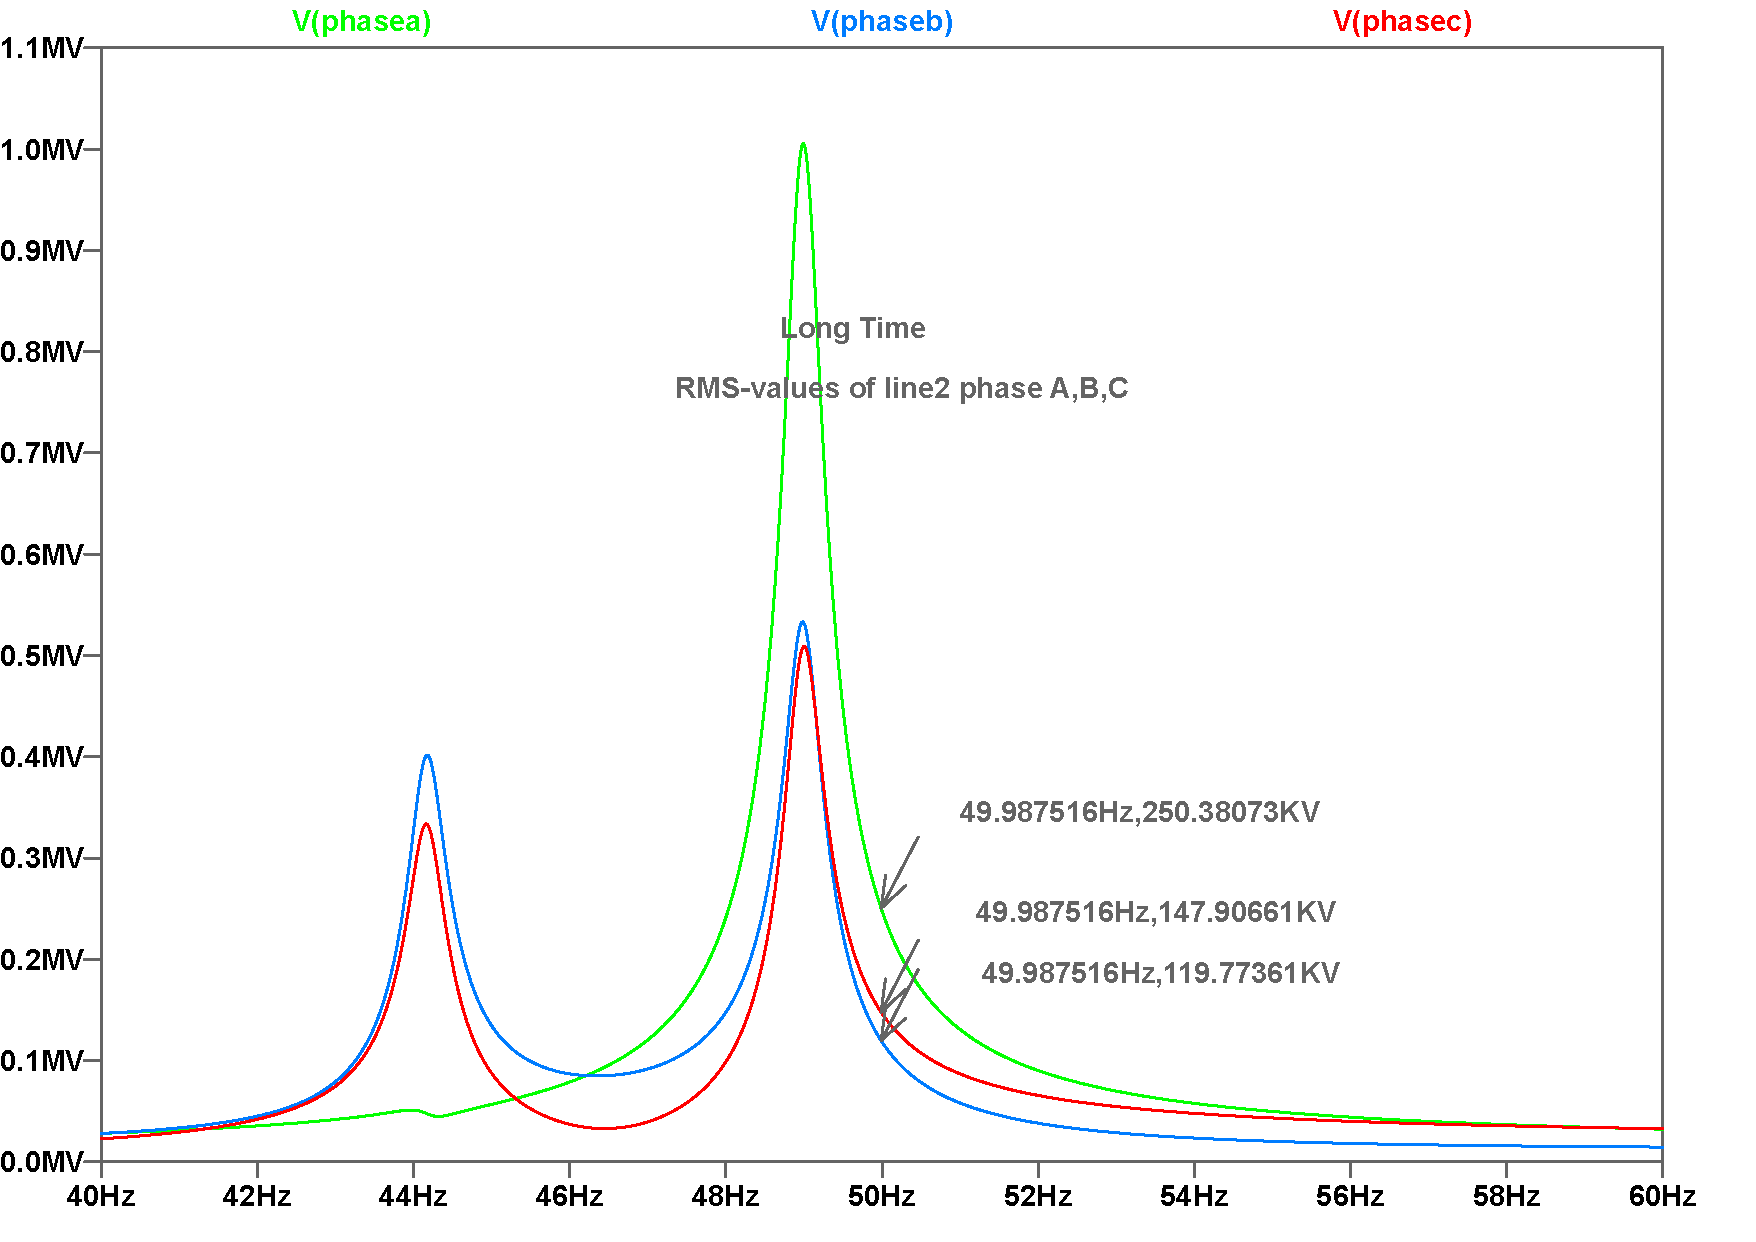
\includegraphics[width=0.90\textwidth]{figures/07_Coupled_lines_resonance/Coupled_lines_resonance_AC}
	\caption{Coupled lines resonance AC - Lines2 is open untransposed}
	\label{fig:figure75}
\end{figure}

\begin{figure}[H]
	\centering
	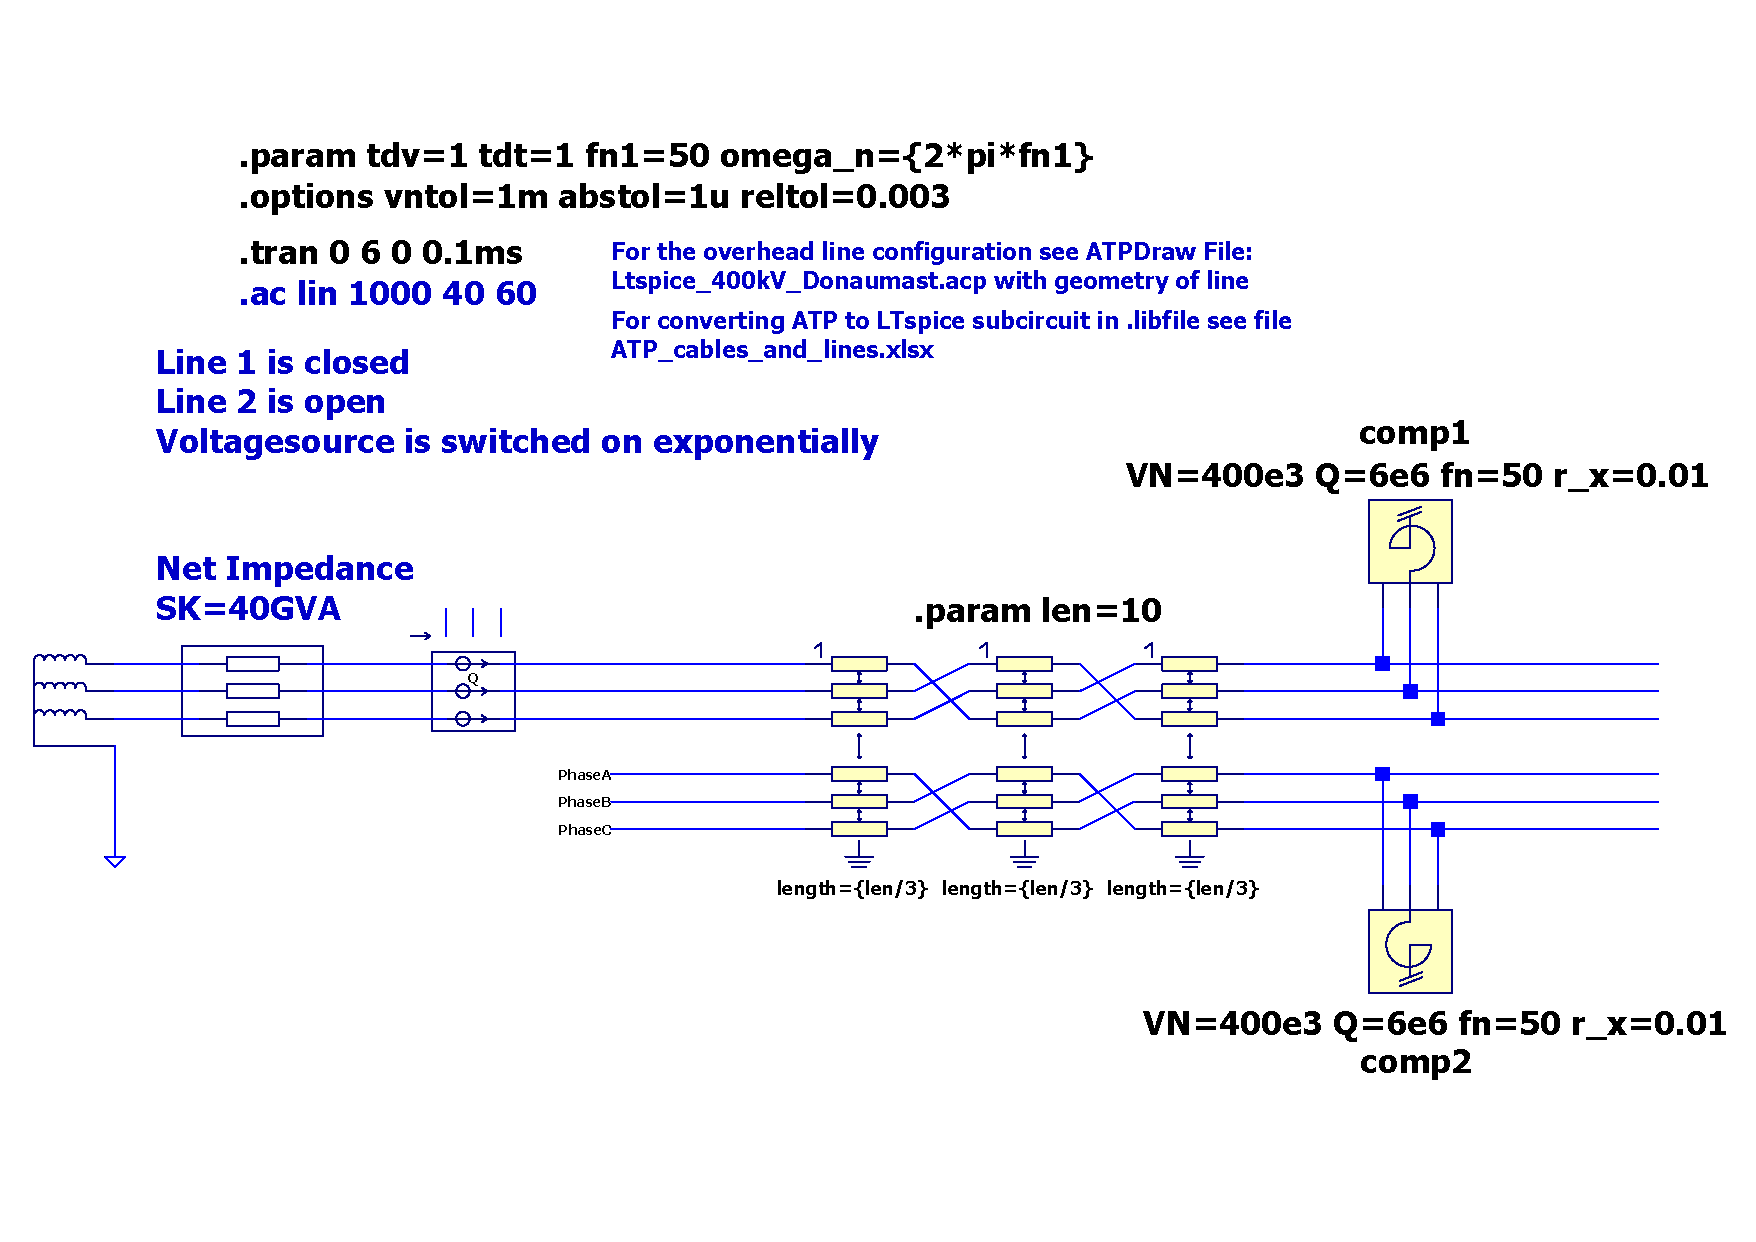
\includegraphics[width=1.0\textwidth]{figures/07_Coupled_lines_resonance/Coupled_lines_resonance_TRAN_transposed_schematic}
	\caption{Coupled lines resonance schematic - Lines2 is open transposed - TRAN analysis}
	\label{fig:figure76}
\end{figure}

\begin{figure}[H]
	\centering
	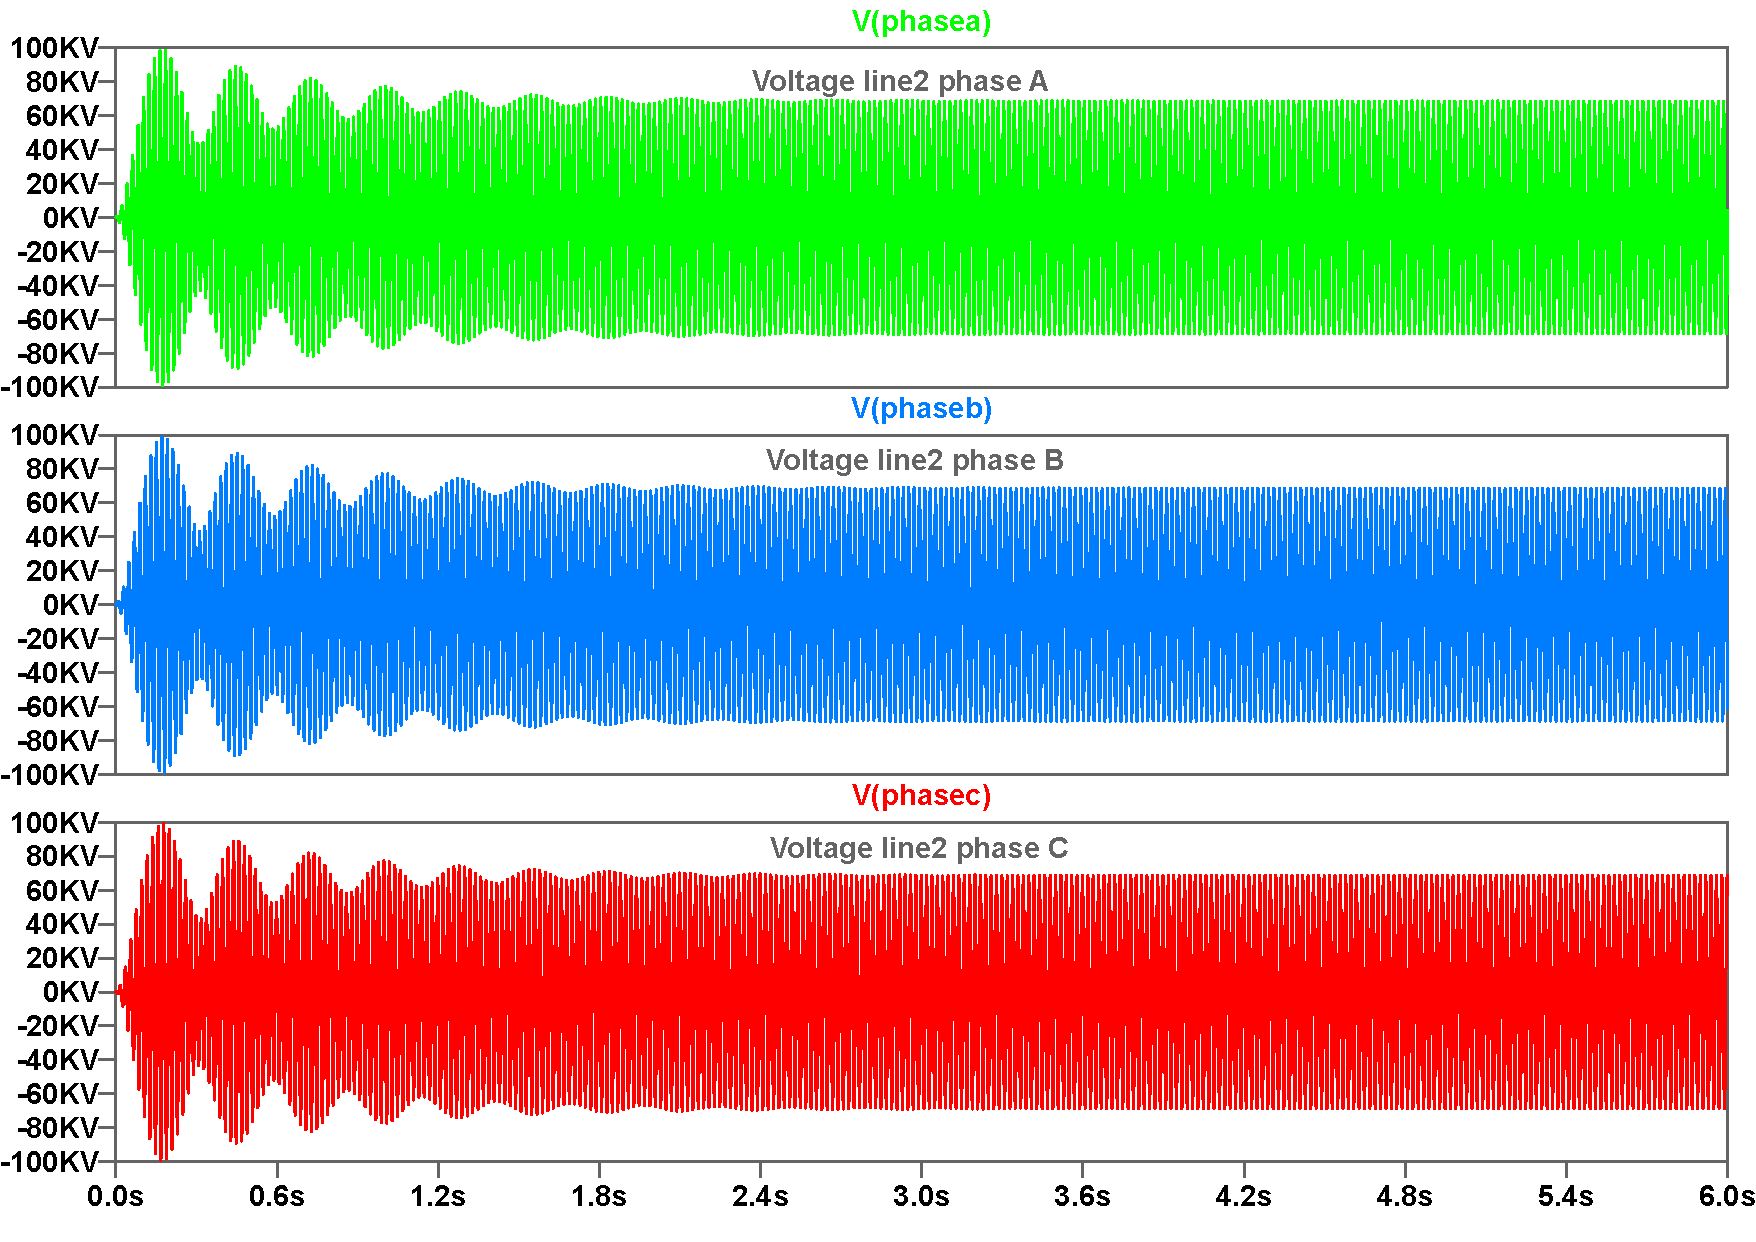
\includegraphics[width=0.90\textwidth]{figures/07_Coupled_lines_resonance/Coupled_lines_resonance_TRAN_transposed}
	\caption{Coupled lines resonance TRAN - Lines2 is open transposed}
	\label{fig:figure77}
\end{figure}

\section{AC Analysis of the Transposed Open Line} figures: \ref{fig:figure78}-\ref{fig:figure79}   (simulation-file: same name as the heading)
\label{sec:coupled-lines-ac-transposed}

The principal resonant peak shifts to approximately \SI{46.3}{\hertz}. The additional
lower-frequency maxima visible in the untransposed model disappear because
the phase coupling has been symmetrized. At \SI{50}{\hertz}, all three phase
voltages are approximately \SI{49}{\kilo\volt} RMS, or
\SI{70}{\kilo\volt} peak, in agreement with the final values of the transient
simulation.

\section{Line 2 Initially Grounded and Then Ungrounded} figures: \ref{fig:figure710}-\ref{fig:figure711}  (simulation-file: same name as the heading)
\label{sec:coupled-line-grounded-then-open}

Line 1 remains energized, while line 2 is initially grounded and subsequently opened.
The final response is similar to the permanently open case in
\cref{sec:coupled-lines-open-untransposed}. A second beat is particularly
visible in Phases A and B; it is associated with the second resonance near
\SI{44}{\hertz} identified by the AC analysis.

\begin{figure}[H]
	\centering
	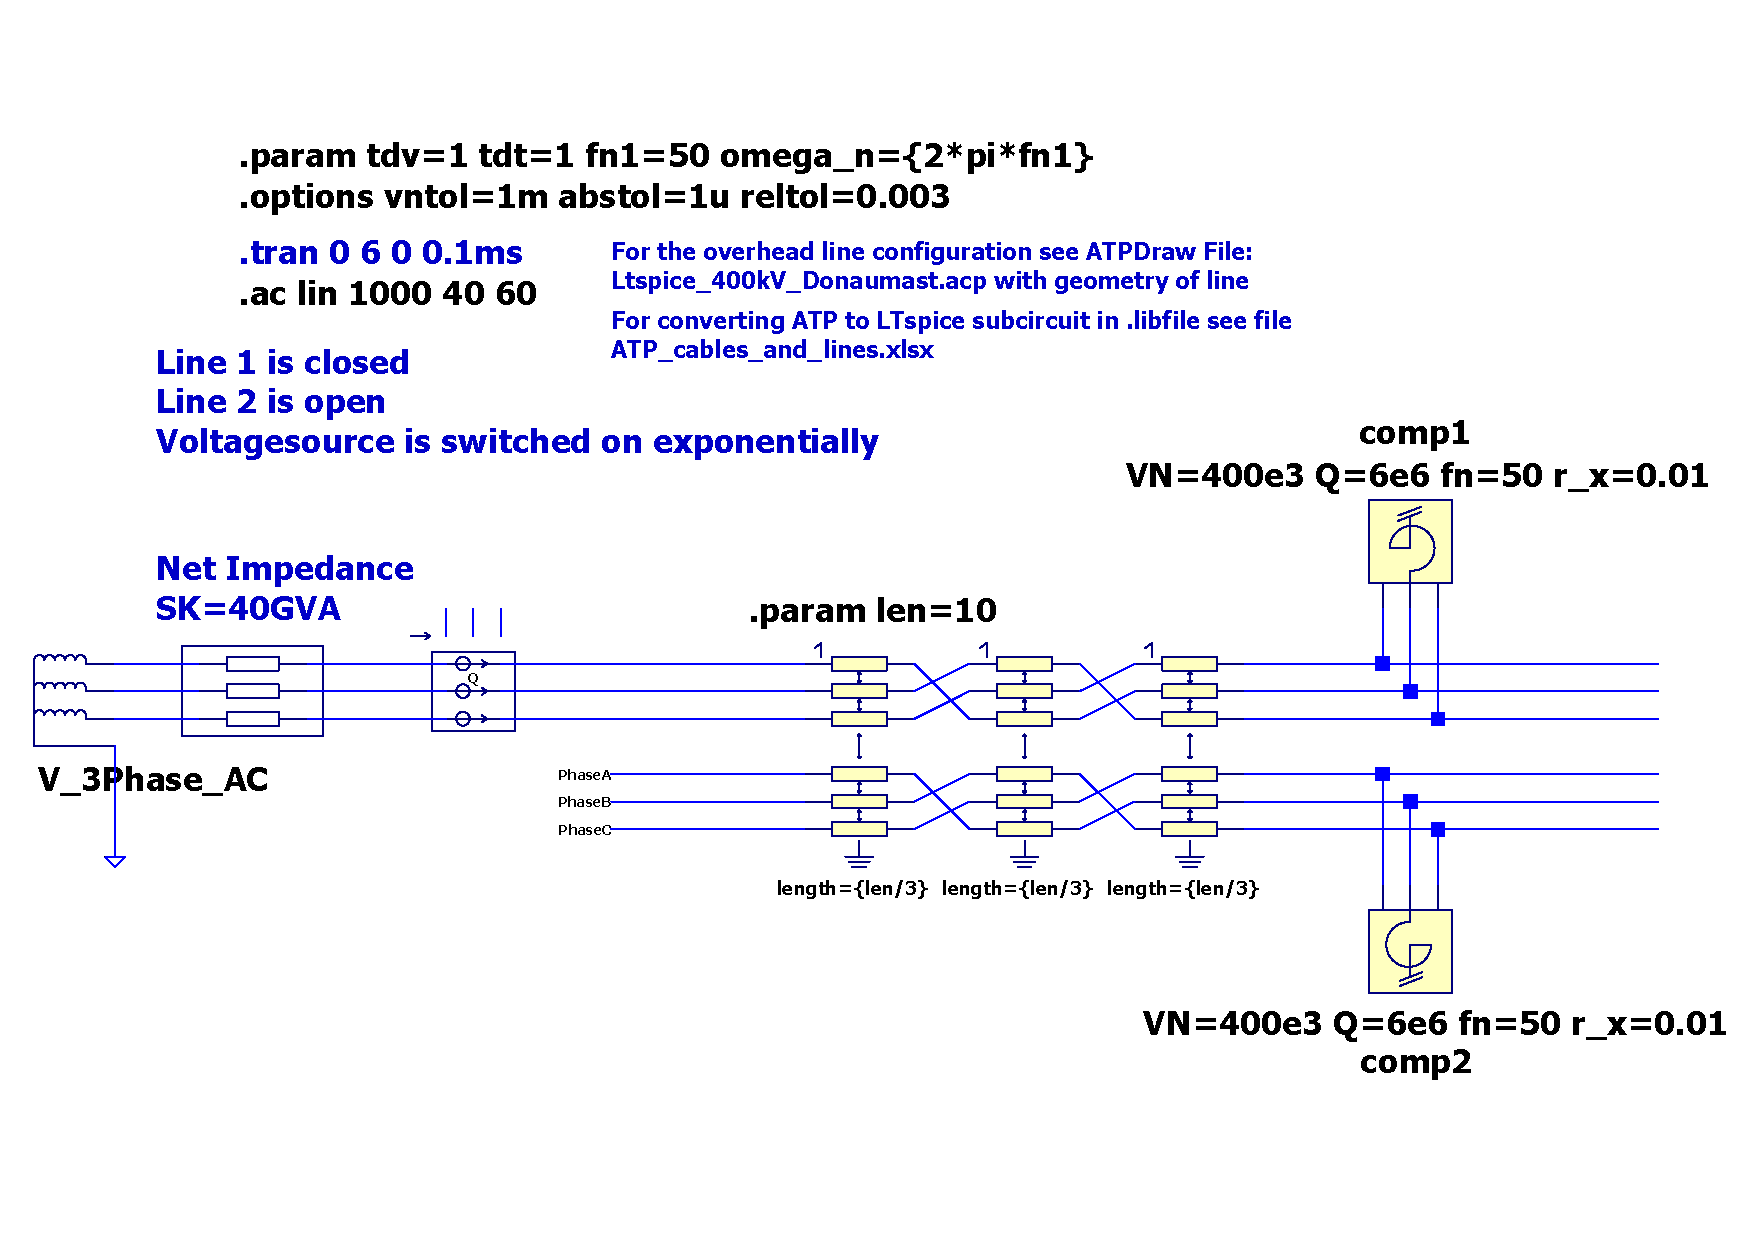
\includegraphics[width=1.0\textwidth]{figures/07_Coupled_lines_resonance/Coupled_lines_resonance_AC_transposed_schematic}
	\caption{Coupled lines resonance schematic Lines2 is open transposed}
	\label{fig:figure78}
\end{figure}

\begin{figure}[H]
	\centering
	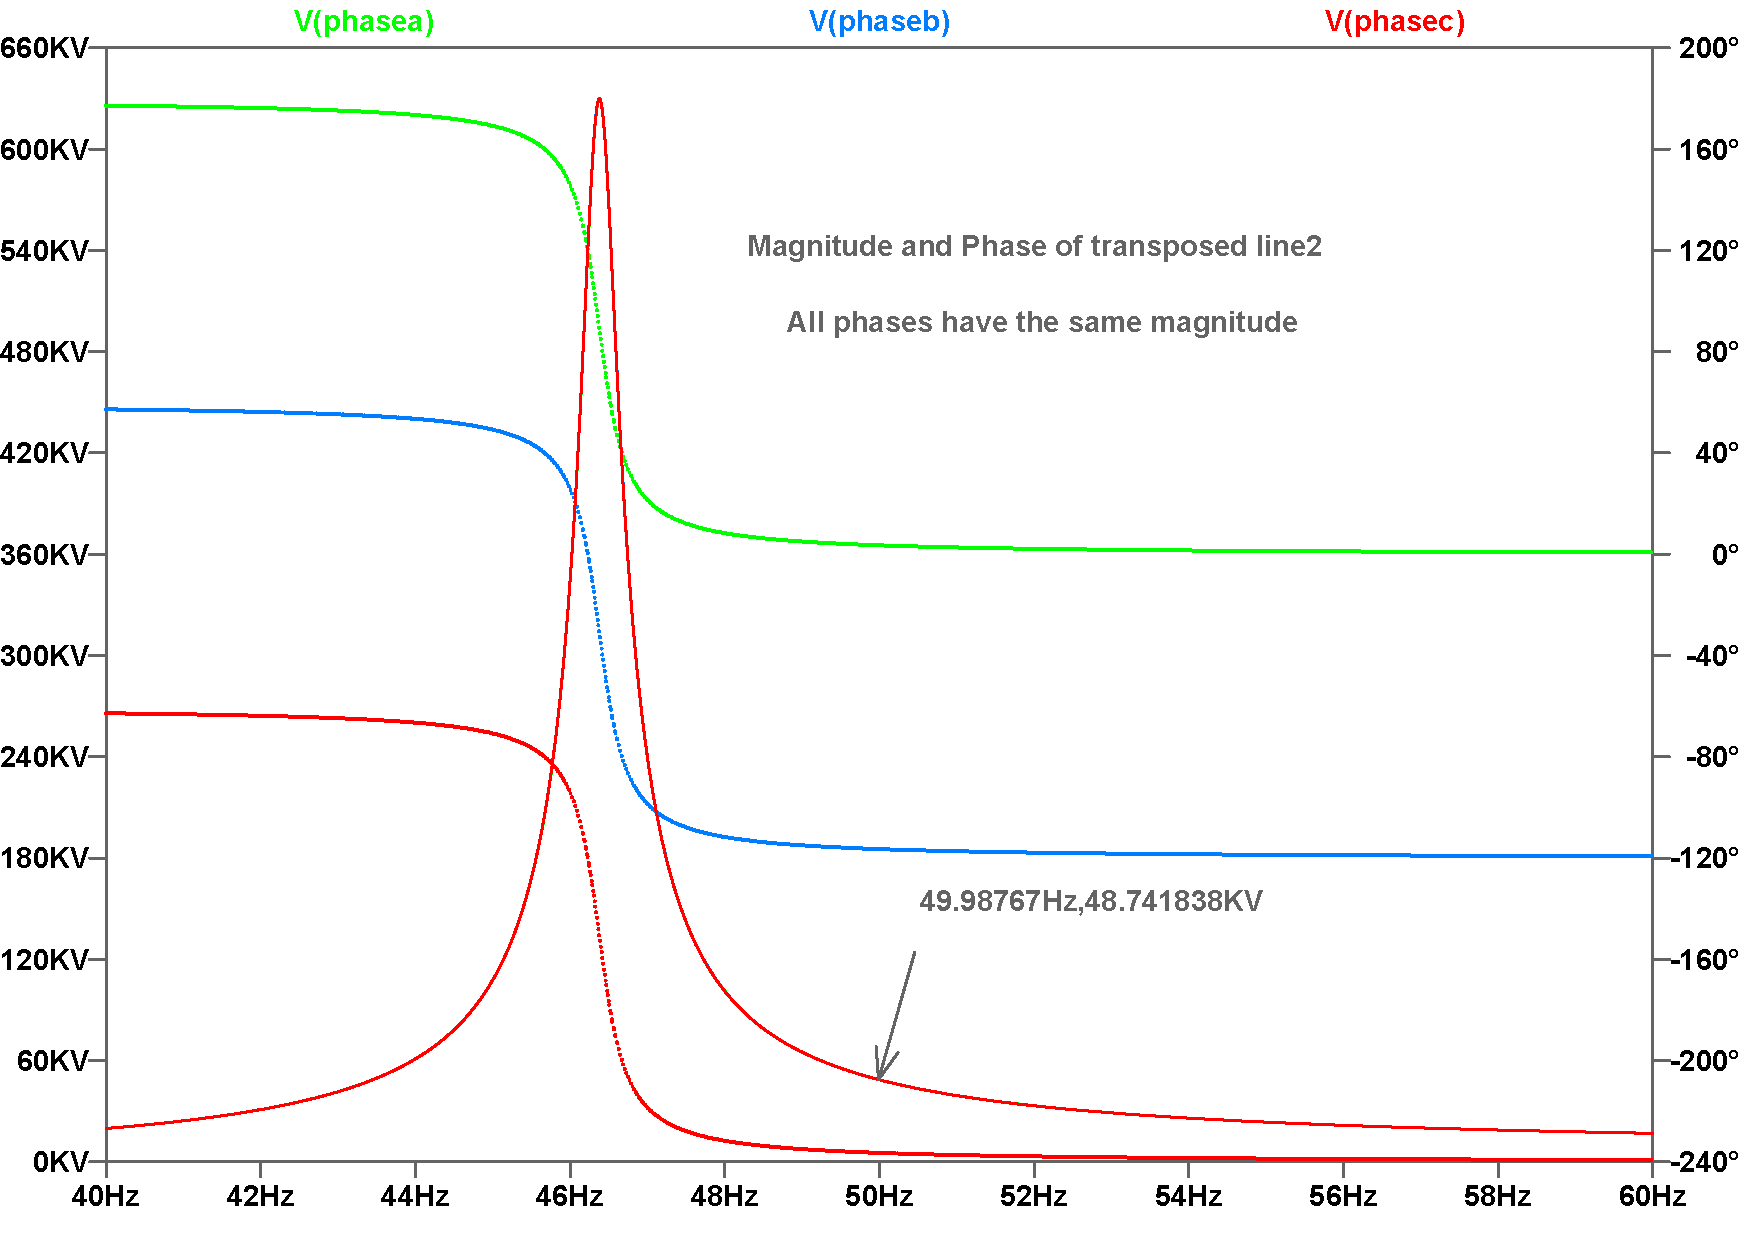
\includegraphics[width=0.90\textwidth]{figures/07_Coupled_lines_resonance/Coupled_lines_resonance_AC_transposed}
	\caption{Coupled lines resonance AC - Lines2 is open transposed}
	\label{fig:figure79}
\end{figure}



\begin{figure}[H]
	\centering
	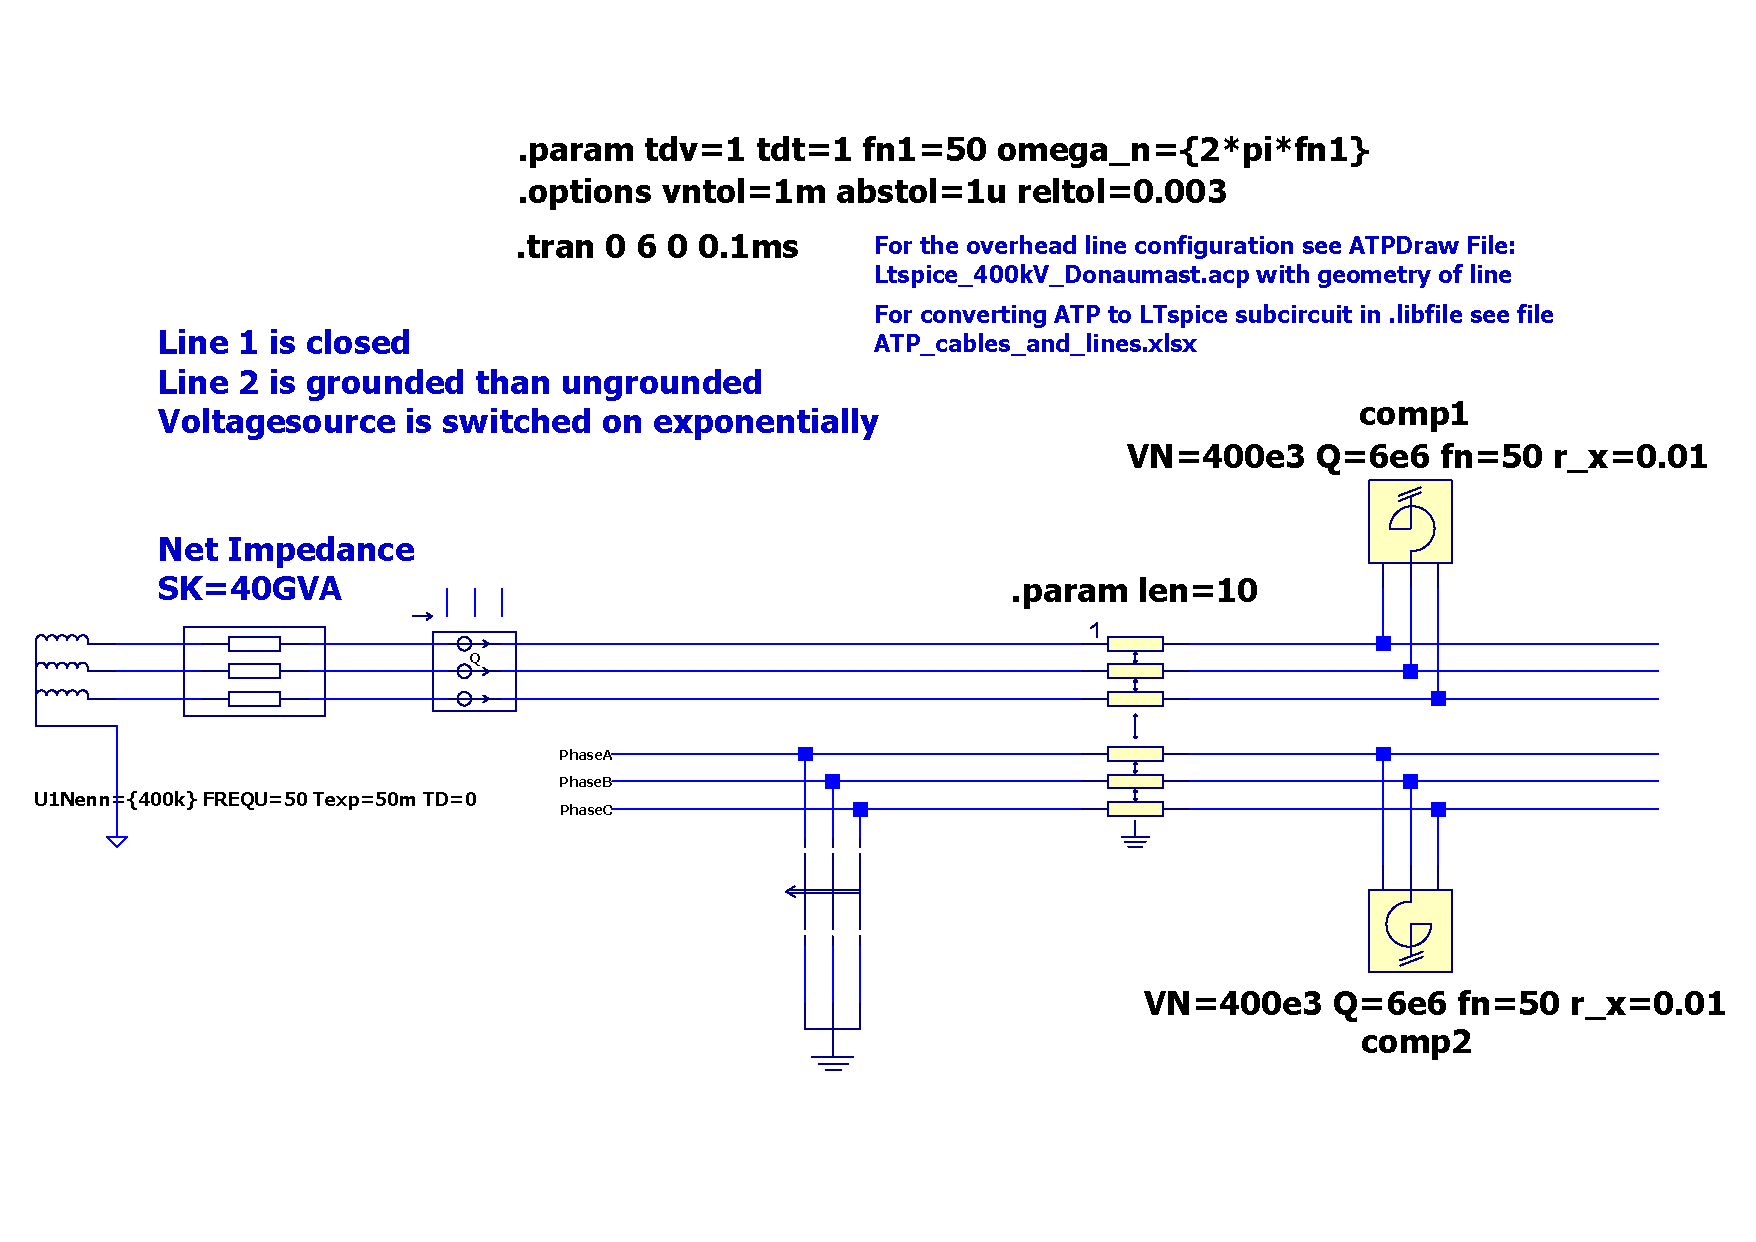
\includegraphics[width=1.0\textwidth]{figures/07_Coupled_lines_resonance/Coupled_lines_resonance_TRAN_grounded_ungrounded_schematic}e
	\caption{Coupled lines resonance TRAN line2 grounded then ungrounded}
	\label{fig:figure710}
\end{figure}

\begin{figure}[H]
	\centering
	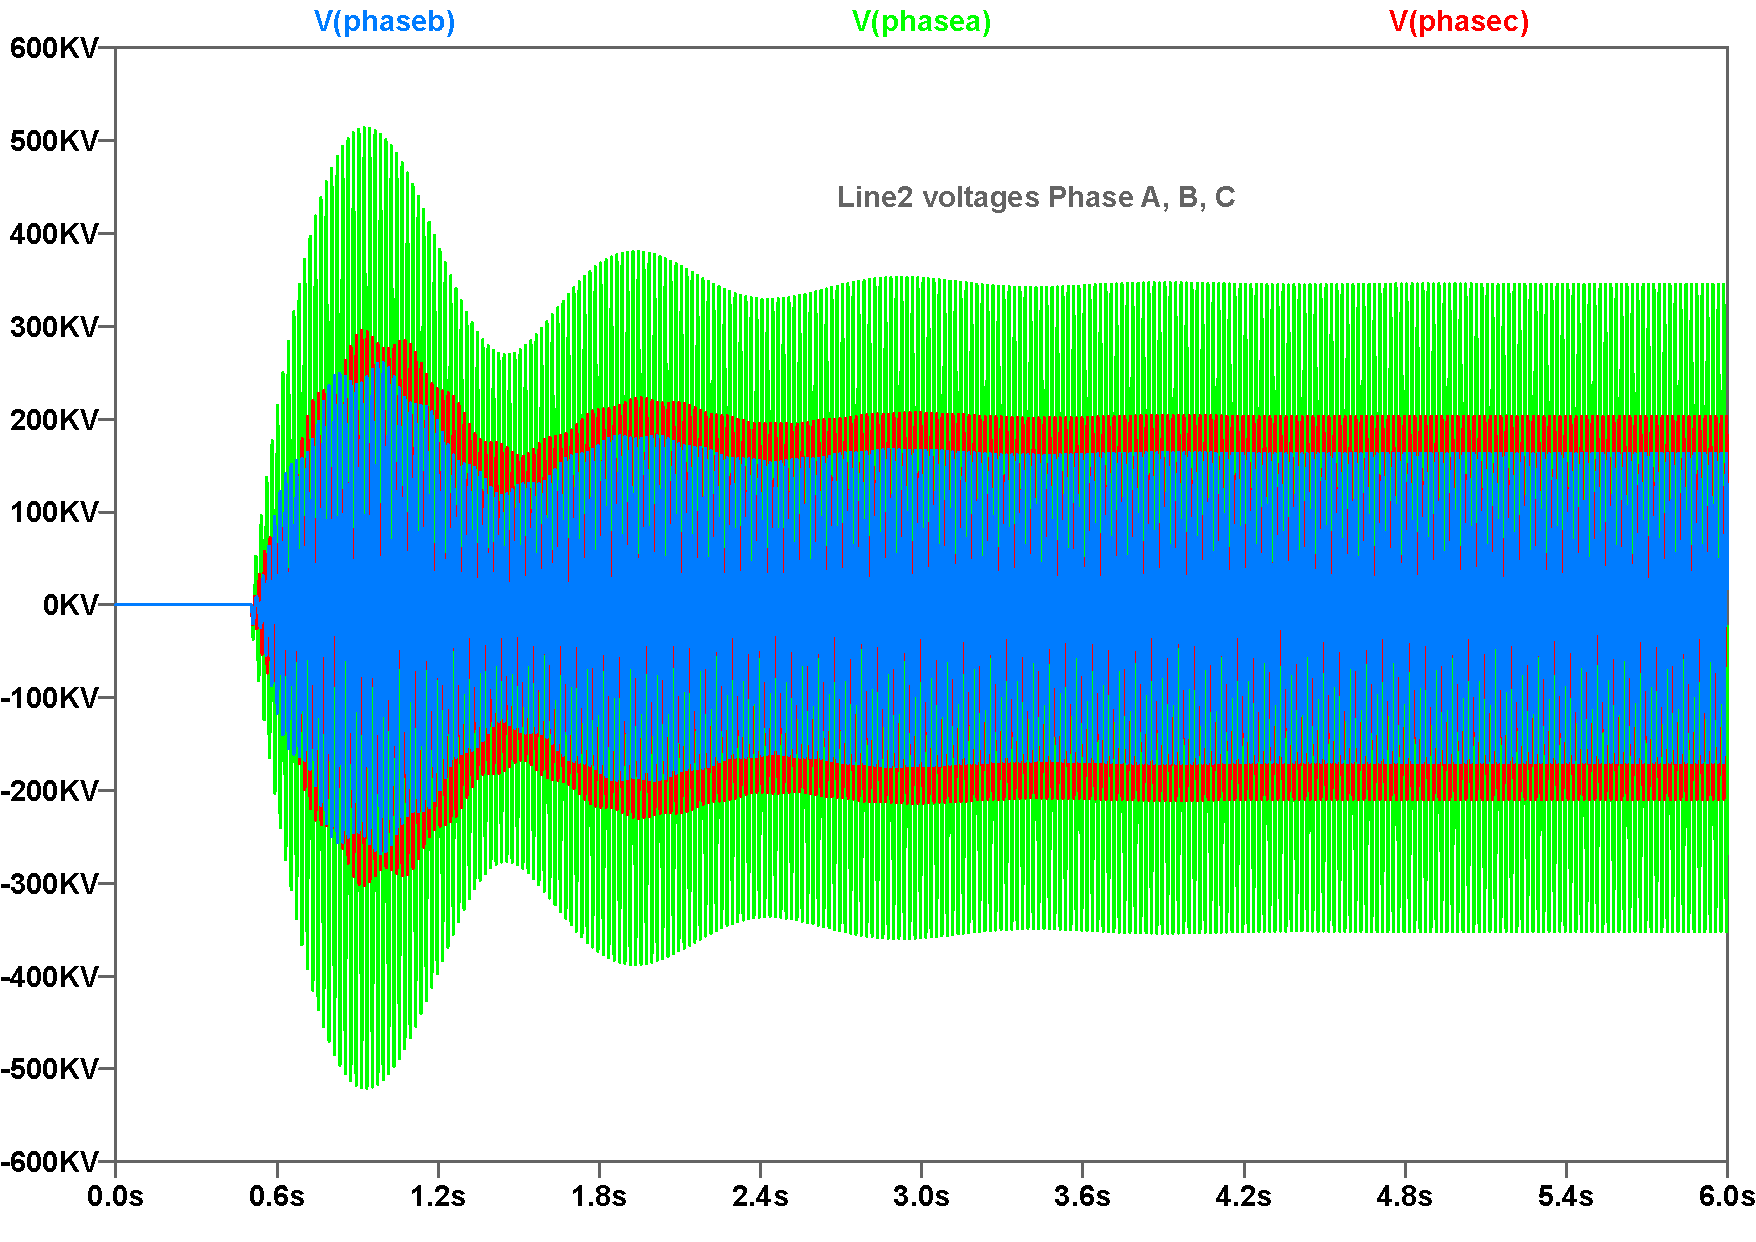
\includegraphics[width=0.90\textwidth]{figures/07_Coupled_lines_resonance/Coupled_lines_resonance_TRAN_grounded_ungrounded}
	\caption{Coupled lines resonance TRAN line2 grounded then ungrounded}
	\label{fig:figure711}
\end{figure}

\section{Line 2 Energized and Subsequently Switched Off} figures: \ref{fig:figure712}-\ref{fig:figure713} (simulation-file: same name as the heading)
\label{sec:coupled-line-switched-off}

Line 2 is disconnected at \SI{500}{\milli\second}. Immediately after opening, its voltage swings to
approximately \SI{-430}{\kilo\volt}. Phase R shows a long-period beat, while
phases B and C show a shorter-period envelope associated with the
\SI{44}{\hertz} resonance.

Select the Phase C voltage and draw a zoom window between two adjacent envelope
maxima. The LTspice status line indicates approximately \SI{5.7}{\hertz}. This
is close to the difference between the source frequency and the second natural
frequency:

\begin{equation}
f_{\mathrm{beat}}\approx
 \left|f_{\mathrm s}-f_{\mathrm r,2}\right|
 \approx\left|\SI{50}{\hertz}-\SI{44}{\hertz}\right|
 \approx\SI{6}{\hertz}.
\end{equation}

\begin{remark}{Exercise}{imp:coupled-line-opening-time}
Save the model as \texttt{test.asc}, change the opening time to
\SI{0.510}{\second}, and compare the phase-voltage peaks. The trapped initial
conditions at the switching instant strongly influence the subsequent free
oscillation.
\end{remark}

\section{Line 2 Switched Off Without a Shunt-Reactor} figures: \ref{fig:figure714}-\ref{fig:figure715}  (simulation-file: same name as the heading)
\label{sec:coupled-line-open-without-reactor}

After line 2 is switched off, its induced phase-voltage peaks are only approximately
\SIrange{20}{30}{\kilo\volt}. Without the \texttt{l\_batt} element, the
near-power-frequency resonance is absent. 

\begin{figure}[H]
	\centering
	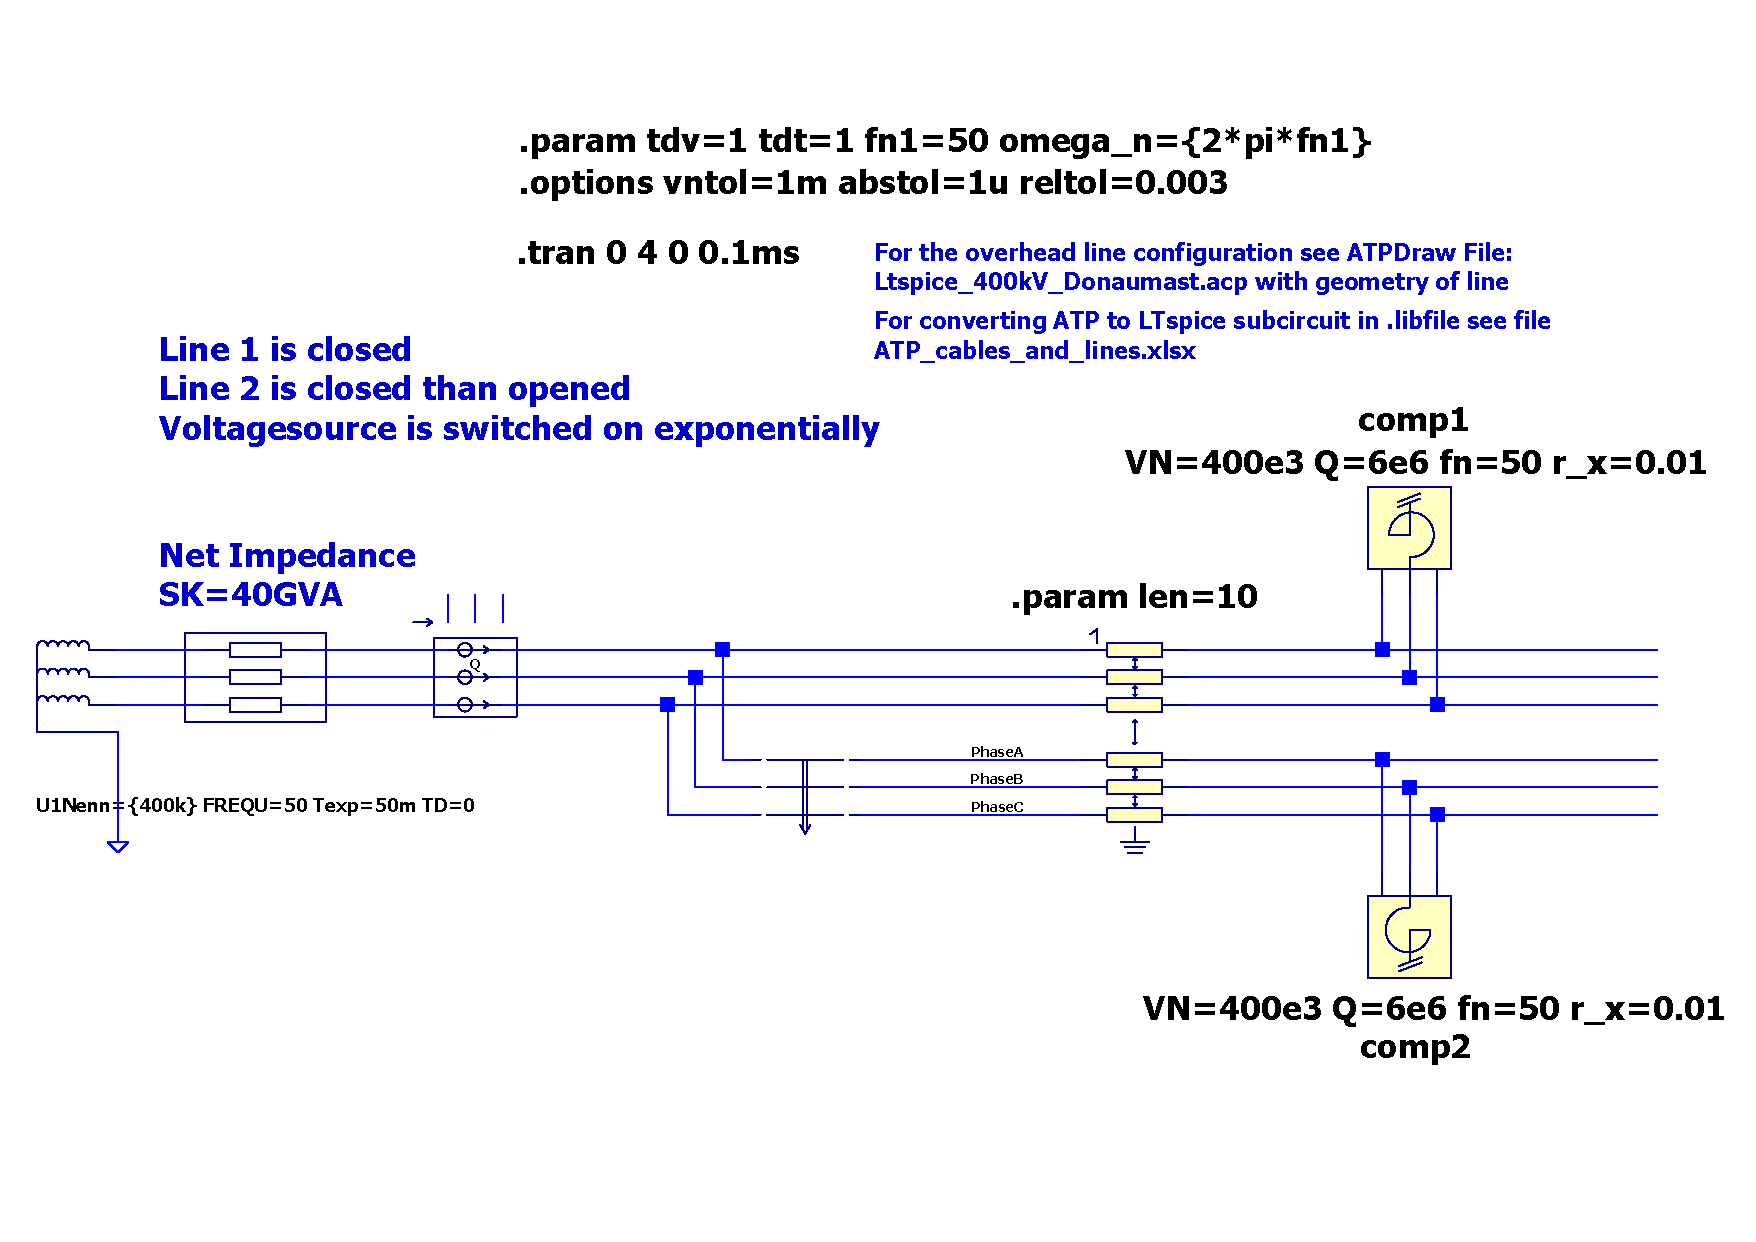
\includegraphics[width=1.0\textwidth]{figures/07_Coupled_lines_resonance/Coupled_lines_resonance_TRAN_switched_off_schematic}
	\caption{Coupled lines resonance TRAN line2 switched off  schematic}
	\label{fig:figure712}
\end{figure}

\begin{figure}[H]
	\centering
	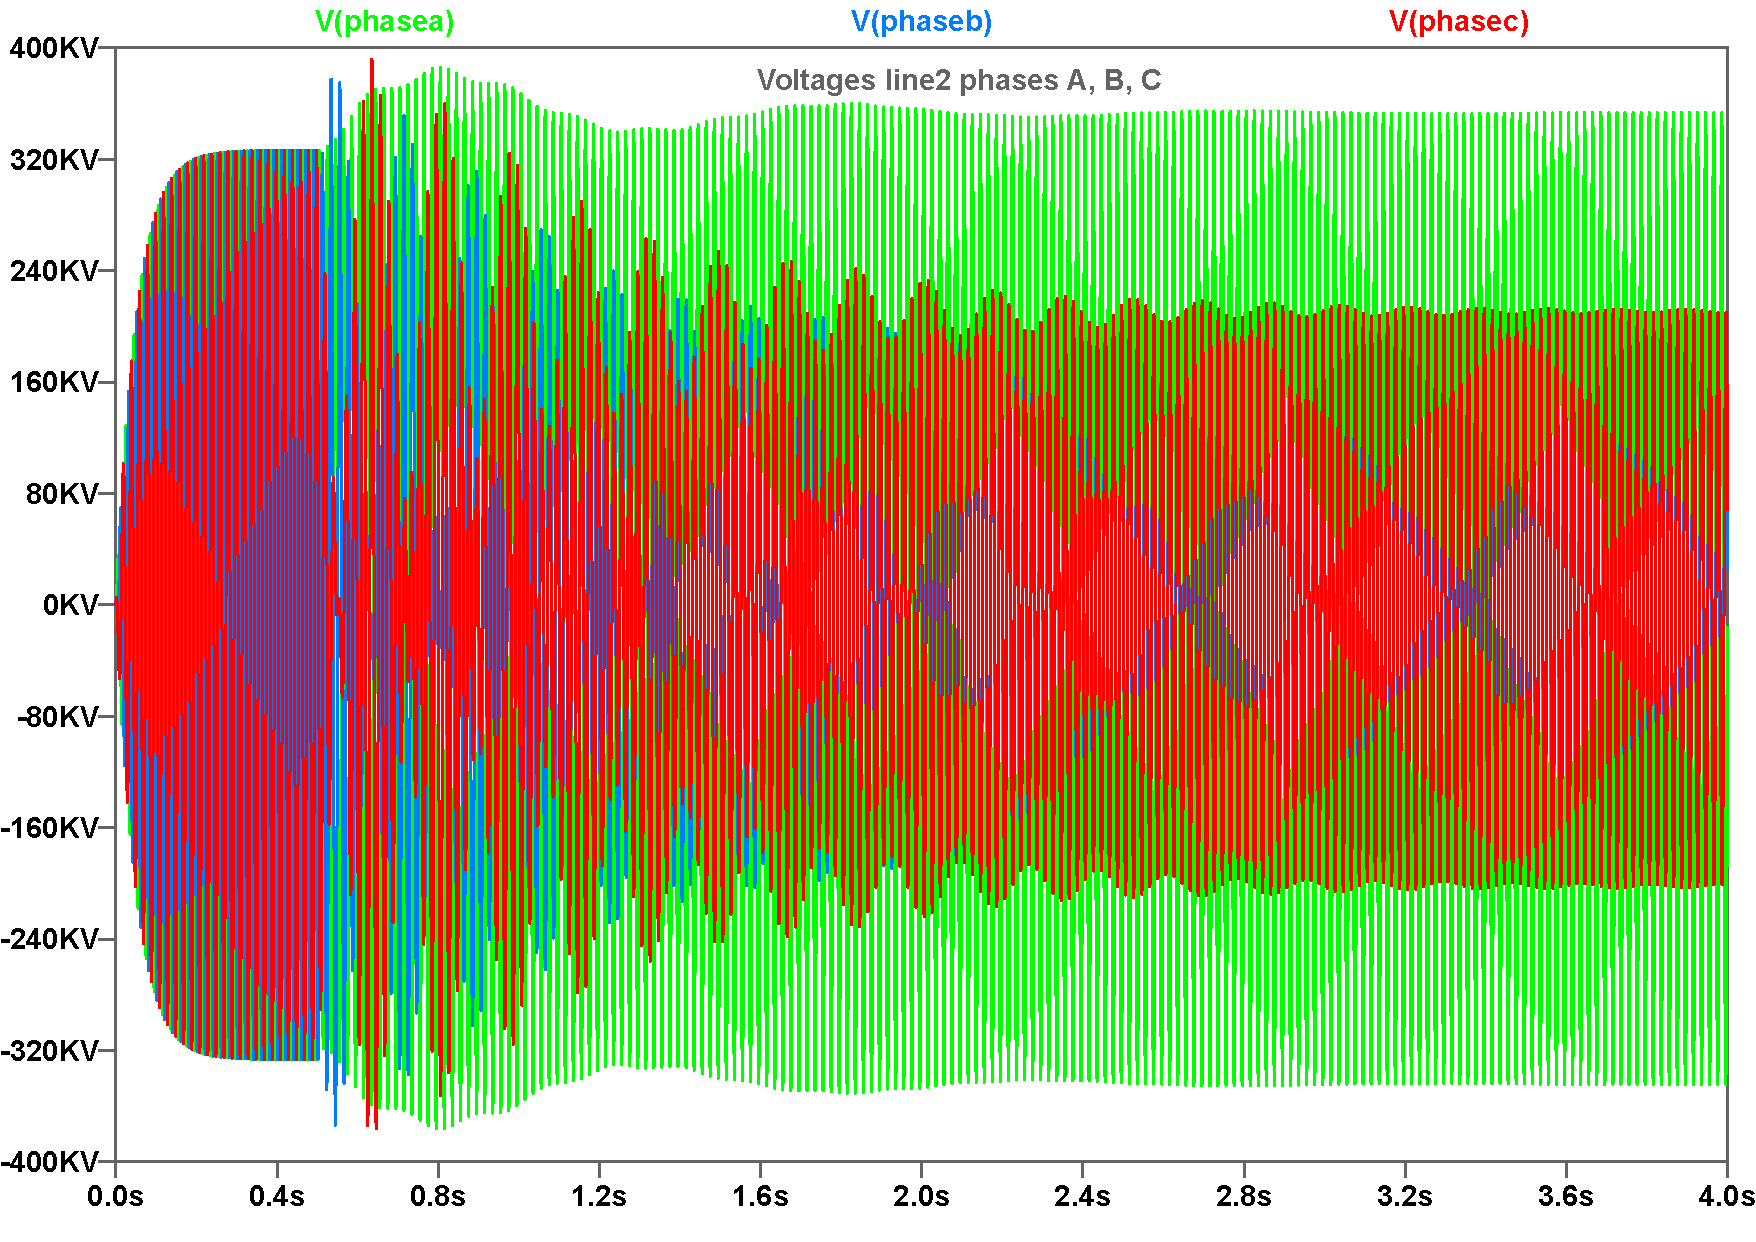
\includegraphics[width=0.90\textwidth]{figures/07_Coupled_lines_resonance/Coupled_lines_resonance_TRAN_switched_off}
	\caption{Coupled lines resonance TRAN line2 switched off}
	\label{fig:figure713}
\end{figure}

\begin{figure}[H]
	\centering
	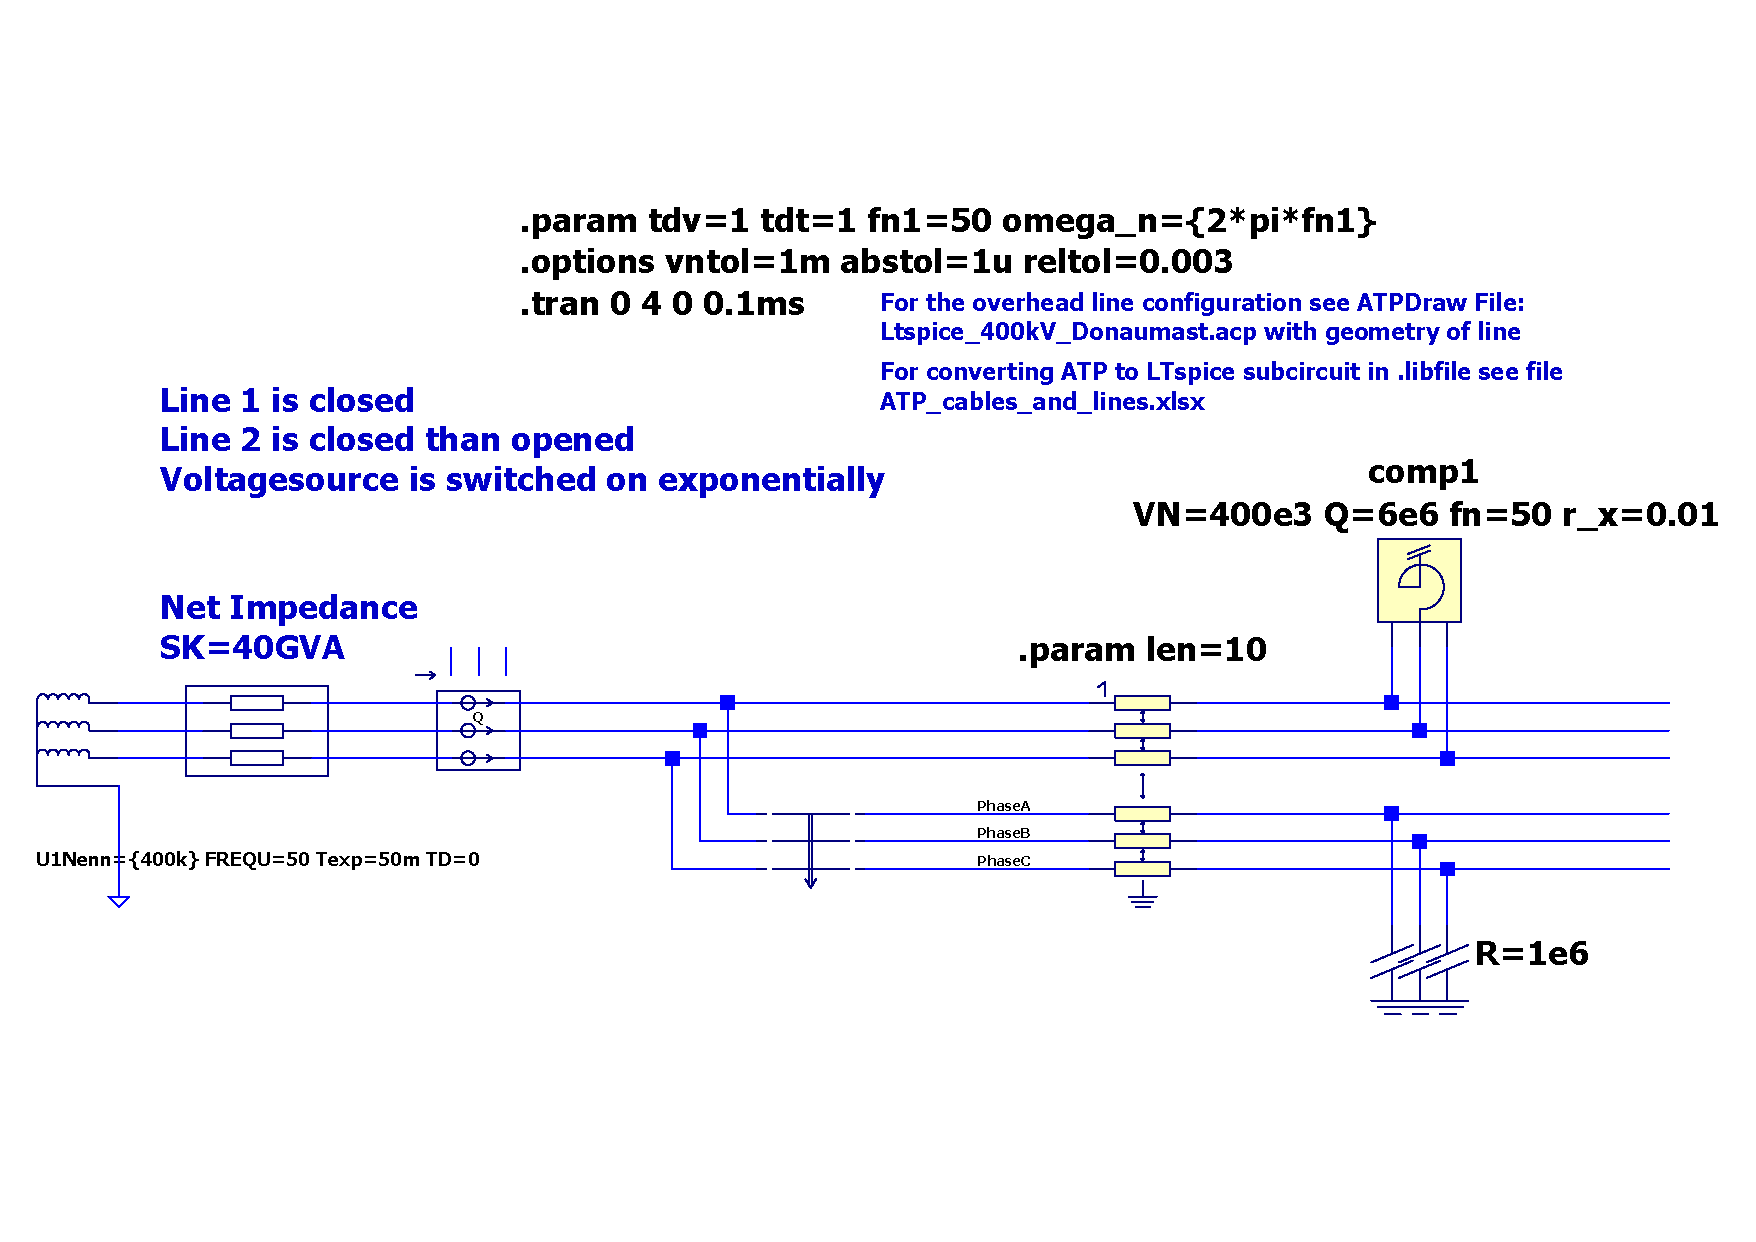
\includegraphics[width=1.0\textwidth]{figures/07_Coupled_lines_resonance/Coupled_lines_resonance_TRAN_switched_off_wo_shuntreactor_schematic}
	\caption{Coupled lines resonance TRAN line2 switched off without shunt reactor schematic }
	\label{fig:figure714}
\end{figure}

\begin{figure}[H]
	\centering
	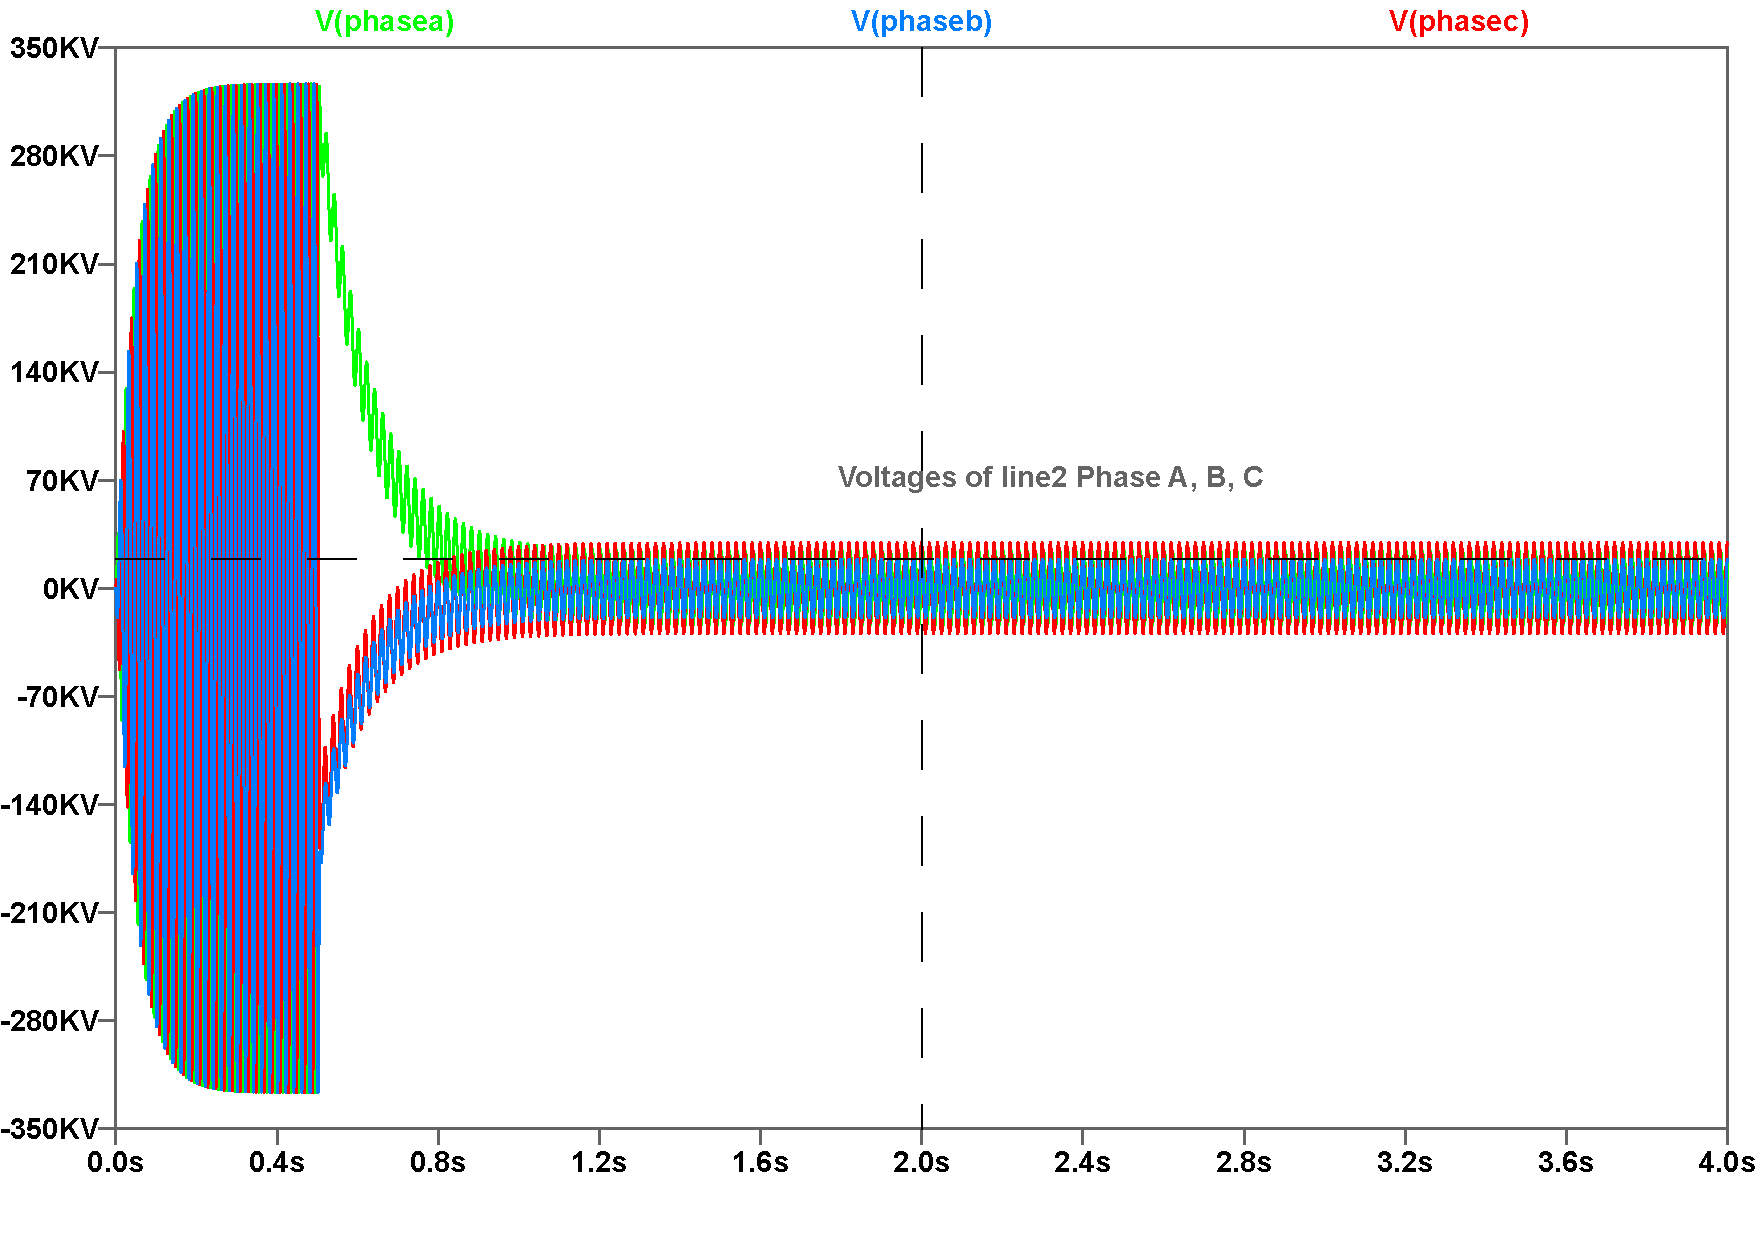
\includegraphics[width=0.90\textwidth]{figures/07_Coupled_lines_resonance/Coupled_lines_resonance_TRAN_switched_off_wo_shuntreactor}
	\caption{Coupled lines resonance TRAN line2 switched off without shunt reactor}
	\label{fig:figure715}
\end{figure}

\section{Stored Energy on the Open Line} figure: 7.16 717 (simulation-file: same name as the heading)
\label{sec:coupled-line-stored-energy}

Line 1 is initially energized and then disconnected. Line 2 is subsequently grounded. To measure
the dissipated energy, hold \textsc{Alt} and click the grounding element, then
hold \textsc{Ctrl} and click the generated power trace. LTspice integrates the
power and displays the corresponding energy. 
NOTE: In this case, the energy should be measured from 1 s to 2 s. Zoom into or set the x-axis to the interval from 1 s to 2 s. During this interval, the stored energy decreases substantially after the line is switched off
After two seconds, only the energy transfer from Line 1 to Line 2 via capacitive coupling between both lines remains. 
This (small) energy should not be included in the measurement.     

The energy released from line 2 is approximately \SI{2.2}{\kilo\joule}.
The stored energy is therefore comparatively small.
With a grounding resistance of \SI{100}{\ohm}, the open-line voltage collapses
almost immediately. It also collapses with \SI{10}{\kilo\ohm}, showing that
the mutual coupling path to line 1 is relatively high-impedance at
\SI{50}{\hertz}.

\begin{figure}[H]
	\centering
	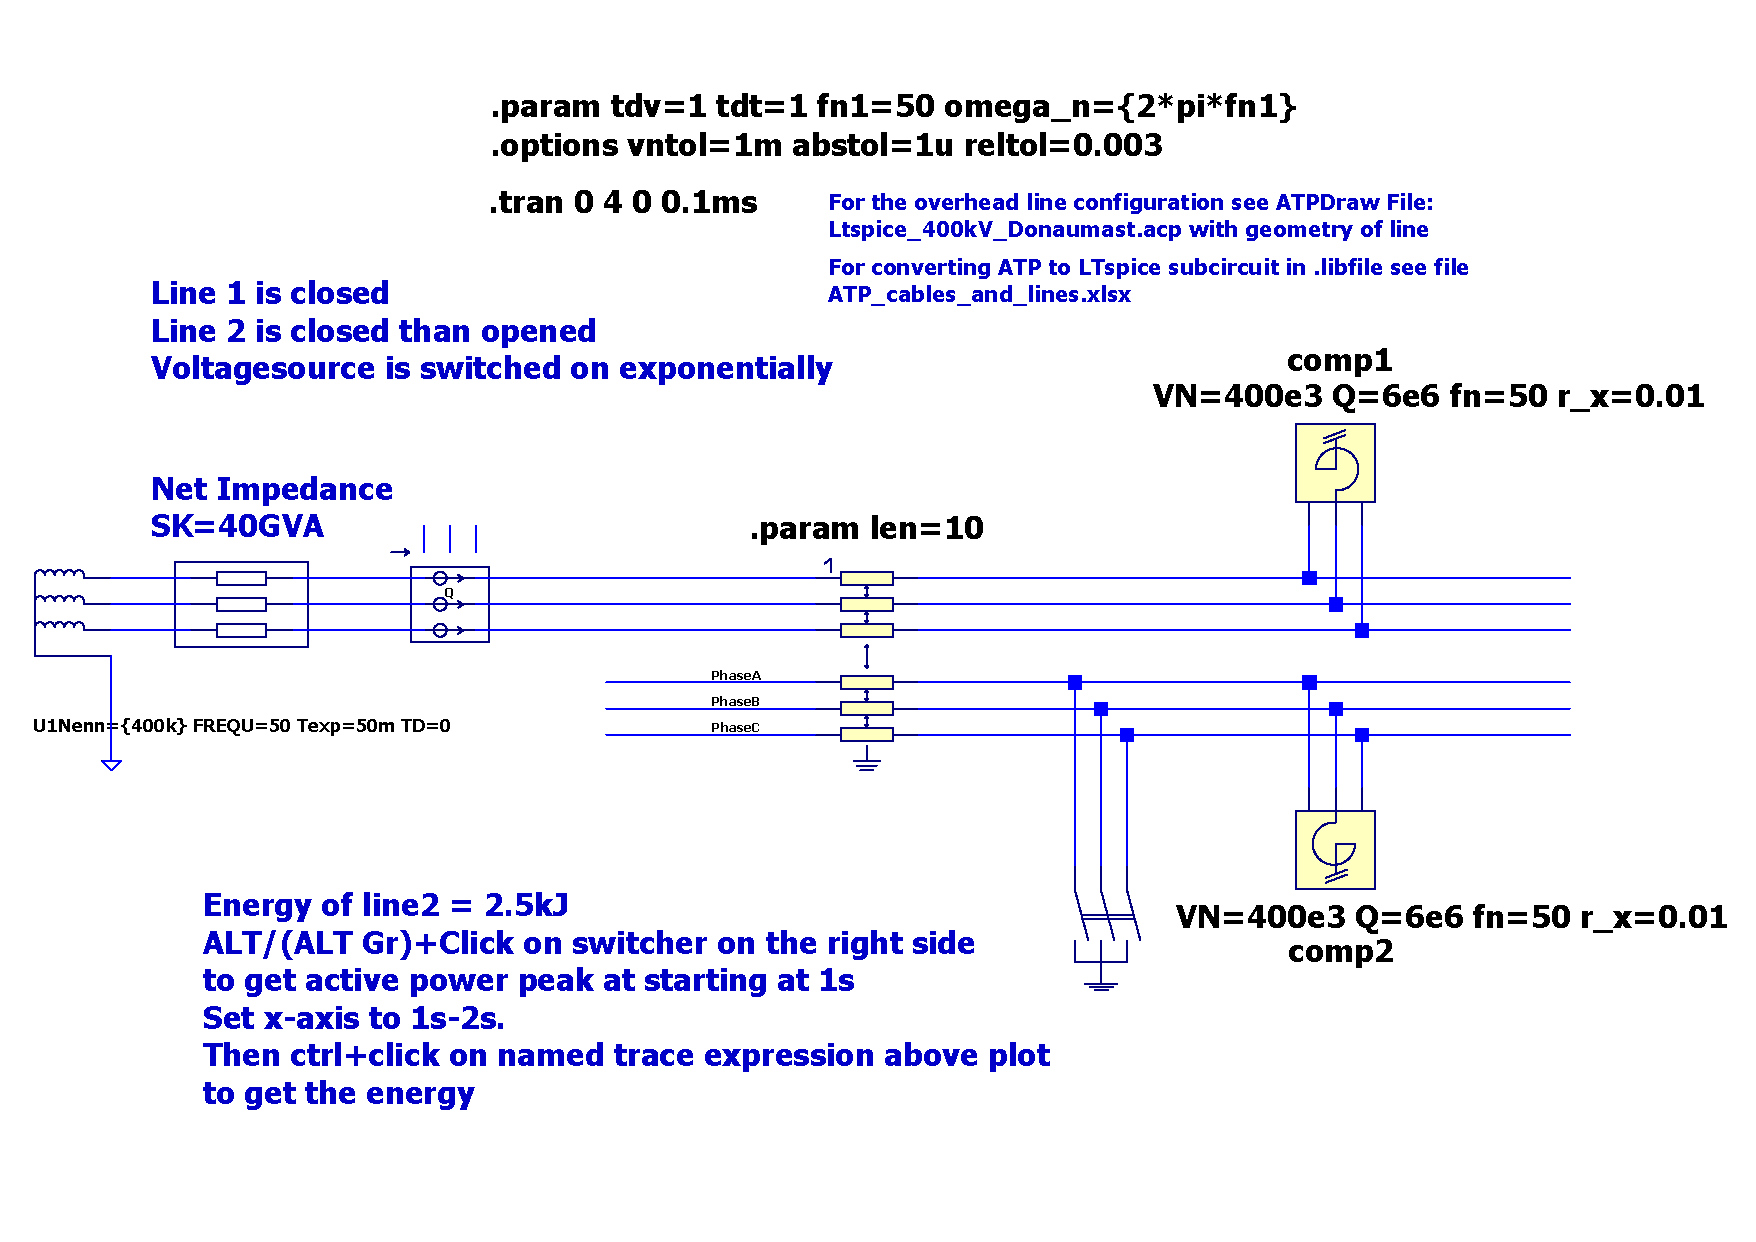
\includegraphics[width=1.0\textwidth]{figures/07_Coupled_lines_resonance/Coupled_lines_resonance_TRAN_stored_energy_schematic}
	\caption{Coupled lines resonance TRAN line2 stored energy schematic }
	\label{fig:figure716}
\end{figure}

\begin{figure}[H]
	\centering
	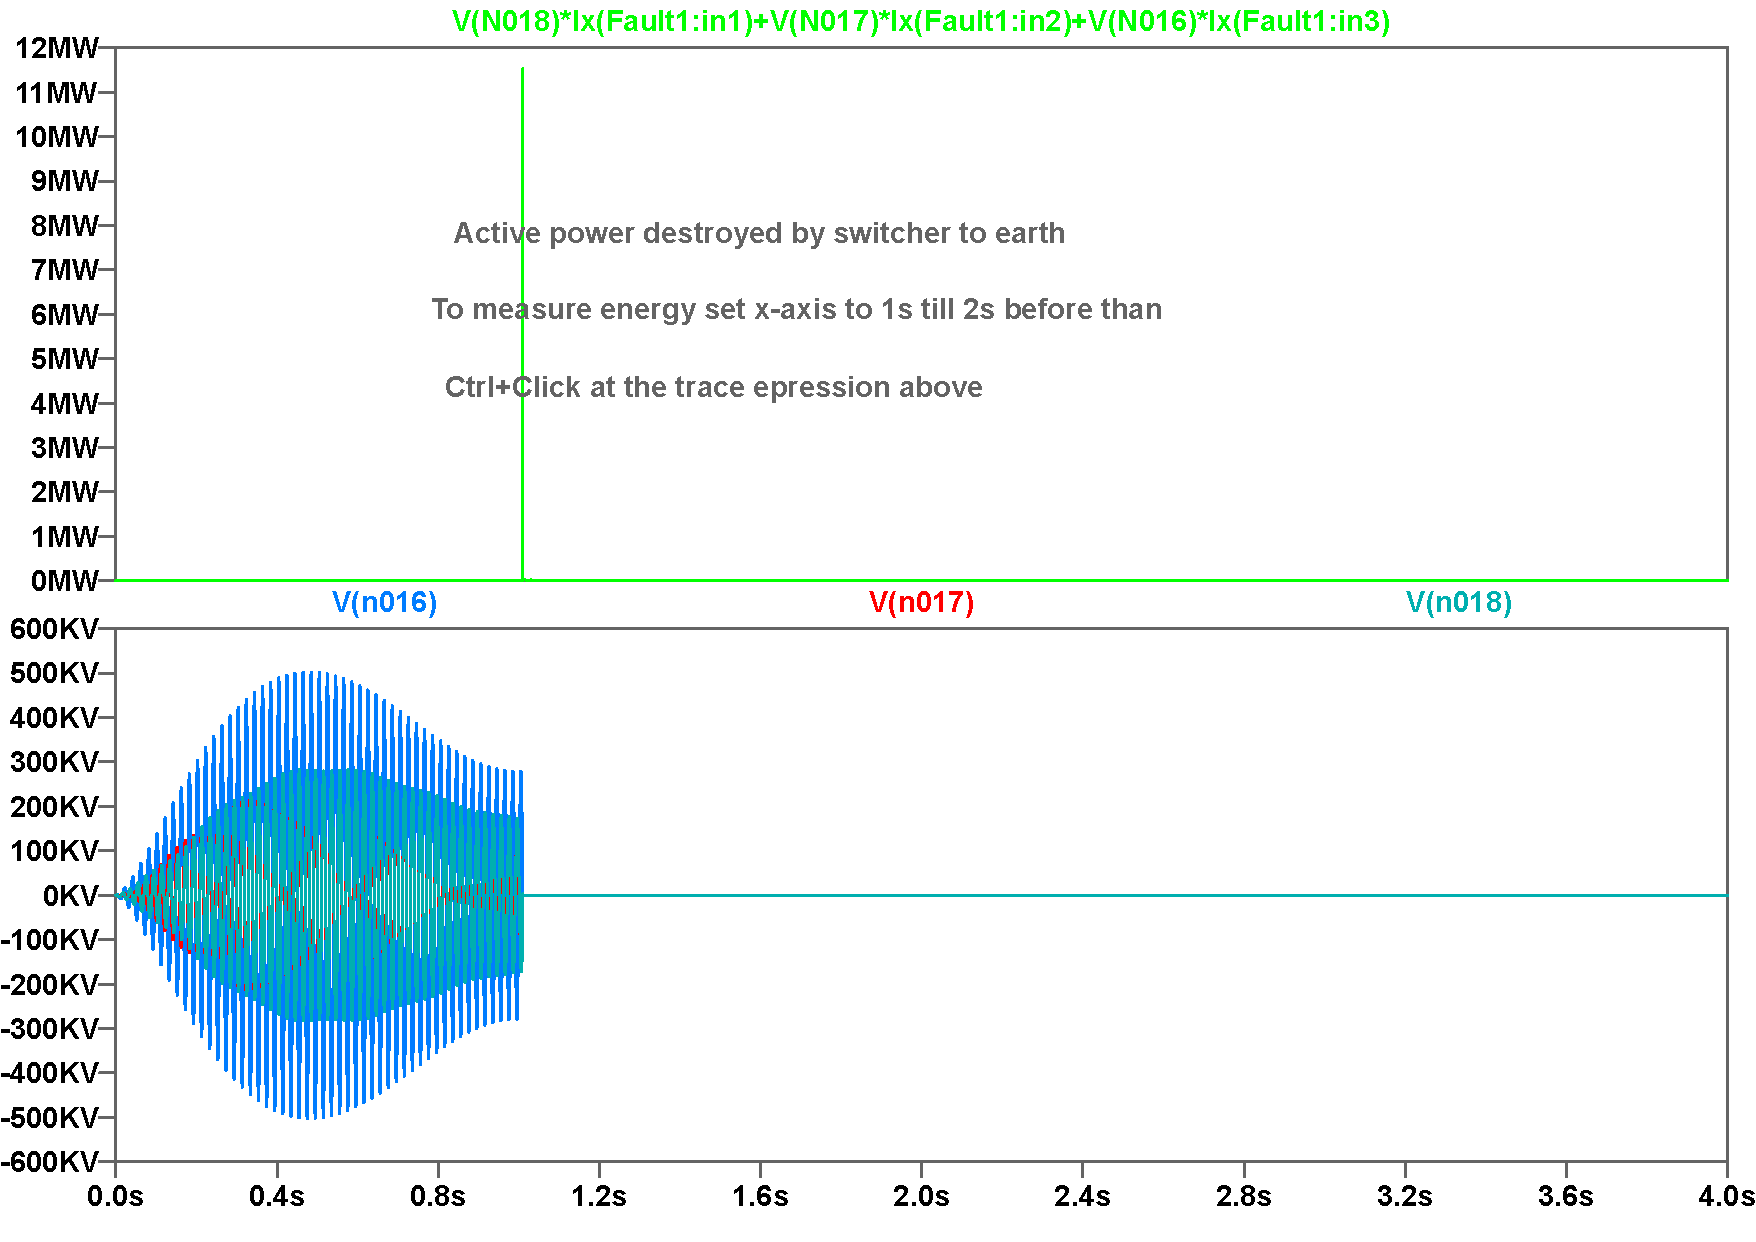
\includegraphics[width=0.90\textwidth]{figures/07_Coupled_lines_resonance/Coupled_lines_resonance_TRAN_stored_energy}
	\caption{Coupled lines resonance TRAN line2 stored energy}
	\label{fig:figure717}
\end{figure}


\begin{chaptersummary}
Mutual inductive and capacitive coupling can impose substantial voltages on an
open overhead-line circuit. Near-exact shunt compensation may place a natural
frequency close to \SI{50}{\hertz} and amplify the open-line voltage to a
dangerous level. Phase transposition symmetrizes the coupling and, in this
example, shifts the resonance away from the operating frequency. Removing the
compensation reactor eliminates the near-power-frequency resonance, while its
loss parameter controls damping.
\end{chaptersummary}
